\documentclass[sensors,article,submit,moreauthors,pdftex]{Definitions/mdpi} 
%=================================================================
\firstpage{1} 
\makeatletter 
\setcounter{page}{\@firstpage} 
\makeatother
\pubvolume{xx}
\issuenum{1}
\articlenumber{5}
\pubyear{2019}
\copyrightyear{2019}
%\externaleditor{Academic Editor: name}
\history{Received: date; Accepted: date; Published: date}
%\updates{yes} % If there is an update available, un-comment this line

%% MDPI internal command: uncomment if new journal that already uses continuous page numbers 
%\continuouspages{yes}

%------------------------------------------------------------------
\usepackage{array}
\usepackage{times}
\usepackage{epsfig}
\usepackage{graphicx}
\usepackage{amsmath}
\usepackage{amssymb}
\usepackage[table]{xcolor}
\usepackage{array}
\usepackage{enumitem}
\usepackage{epsfig} % for postscript graphics files
\usepackage{mathptmx} % assumes new font selection scheme installed
\usepackage{amsfonts}
\usepackage{mdwmath}
\usepackage[caption=false,font=footnotesize]{subfig}
\usepackage{url}
\usepackage{float}
\usepackage[numbers,sort&compress]{natbib}
\usepackage{balance}
\usepackage[english]{babel}
\usepackage[font=footnotesize]{caption}
\usepackage{comment}
\newcommand{\eqnref}[1]{Equation~(\ref{eqn:#1})}
\newcommand{\figref}[1]{Fig.~\ref{fig:#1}}
\newcommand{\tblref}[1]{Table~\ref{tbl:#1}}
\newcommand{\secref}[1]{Section~\ref{sec:#1}}
\newcommand{\algref}[1]{Algorithm.~\ref{alg:#1}}
\newcommand{\com}[1]{\textcolor{red}{#1}}
%%%%%%%%%%%% add files
%========= Method overview
%% trim=left bottom right top
\newcommand{\MethodOverview}{
\begin{figure}[t]
    \centering
    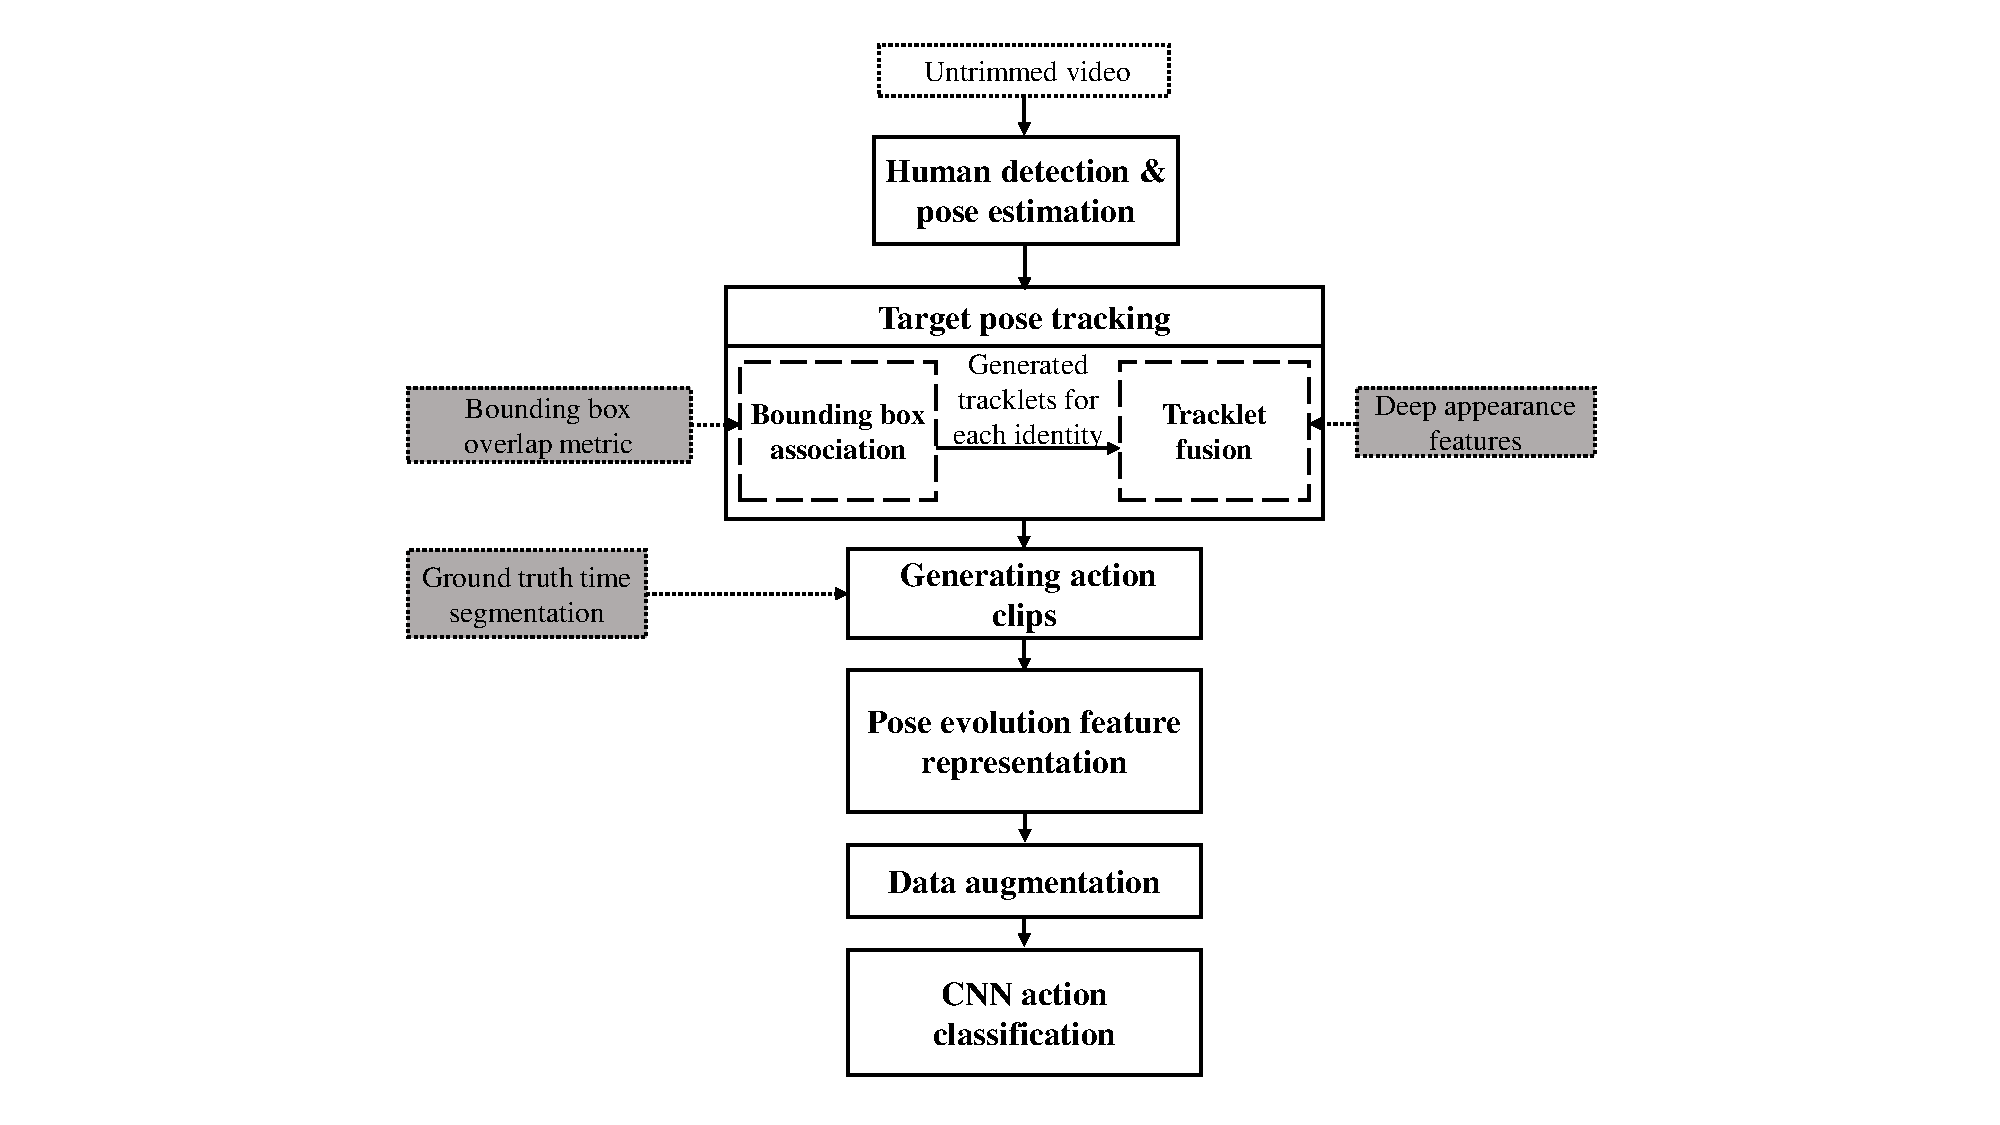
\includegraphics[width=1\linewidth, trim=2.5in 0.0in 2.5in 0.0in, clip=true]{Figures/Method.pdf}
    \caption{Overview of the proposed multi-stage method for human behavior phenotyping in untrimmed videos. At the first stage, human detection and pose estimation is applied on the recorded video. At the second stage, the regressed bounding boxes for each detected person and corresponding keypoints are used for the tracking the identities in video. Tracking is done in an incremental process incorporating both appearance and time information. Outputs of tracking the target identity along with ground-truth time segmentation are used for generating a compact representation of the target actor pose evolution in time for each action clip. Finally, the augmented pose evolution representation is fed to a CNN-based action classification network to recognize actions of interest.}
    \label{fig:Method}
    \vspace{-.1in}
\end{figure}
}
%===============================
\newcommand{\PoseNet}{
\begin{figure*}[ht]
    \centering
    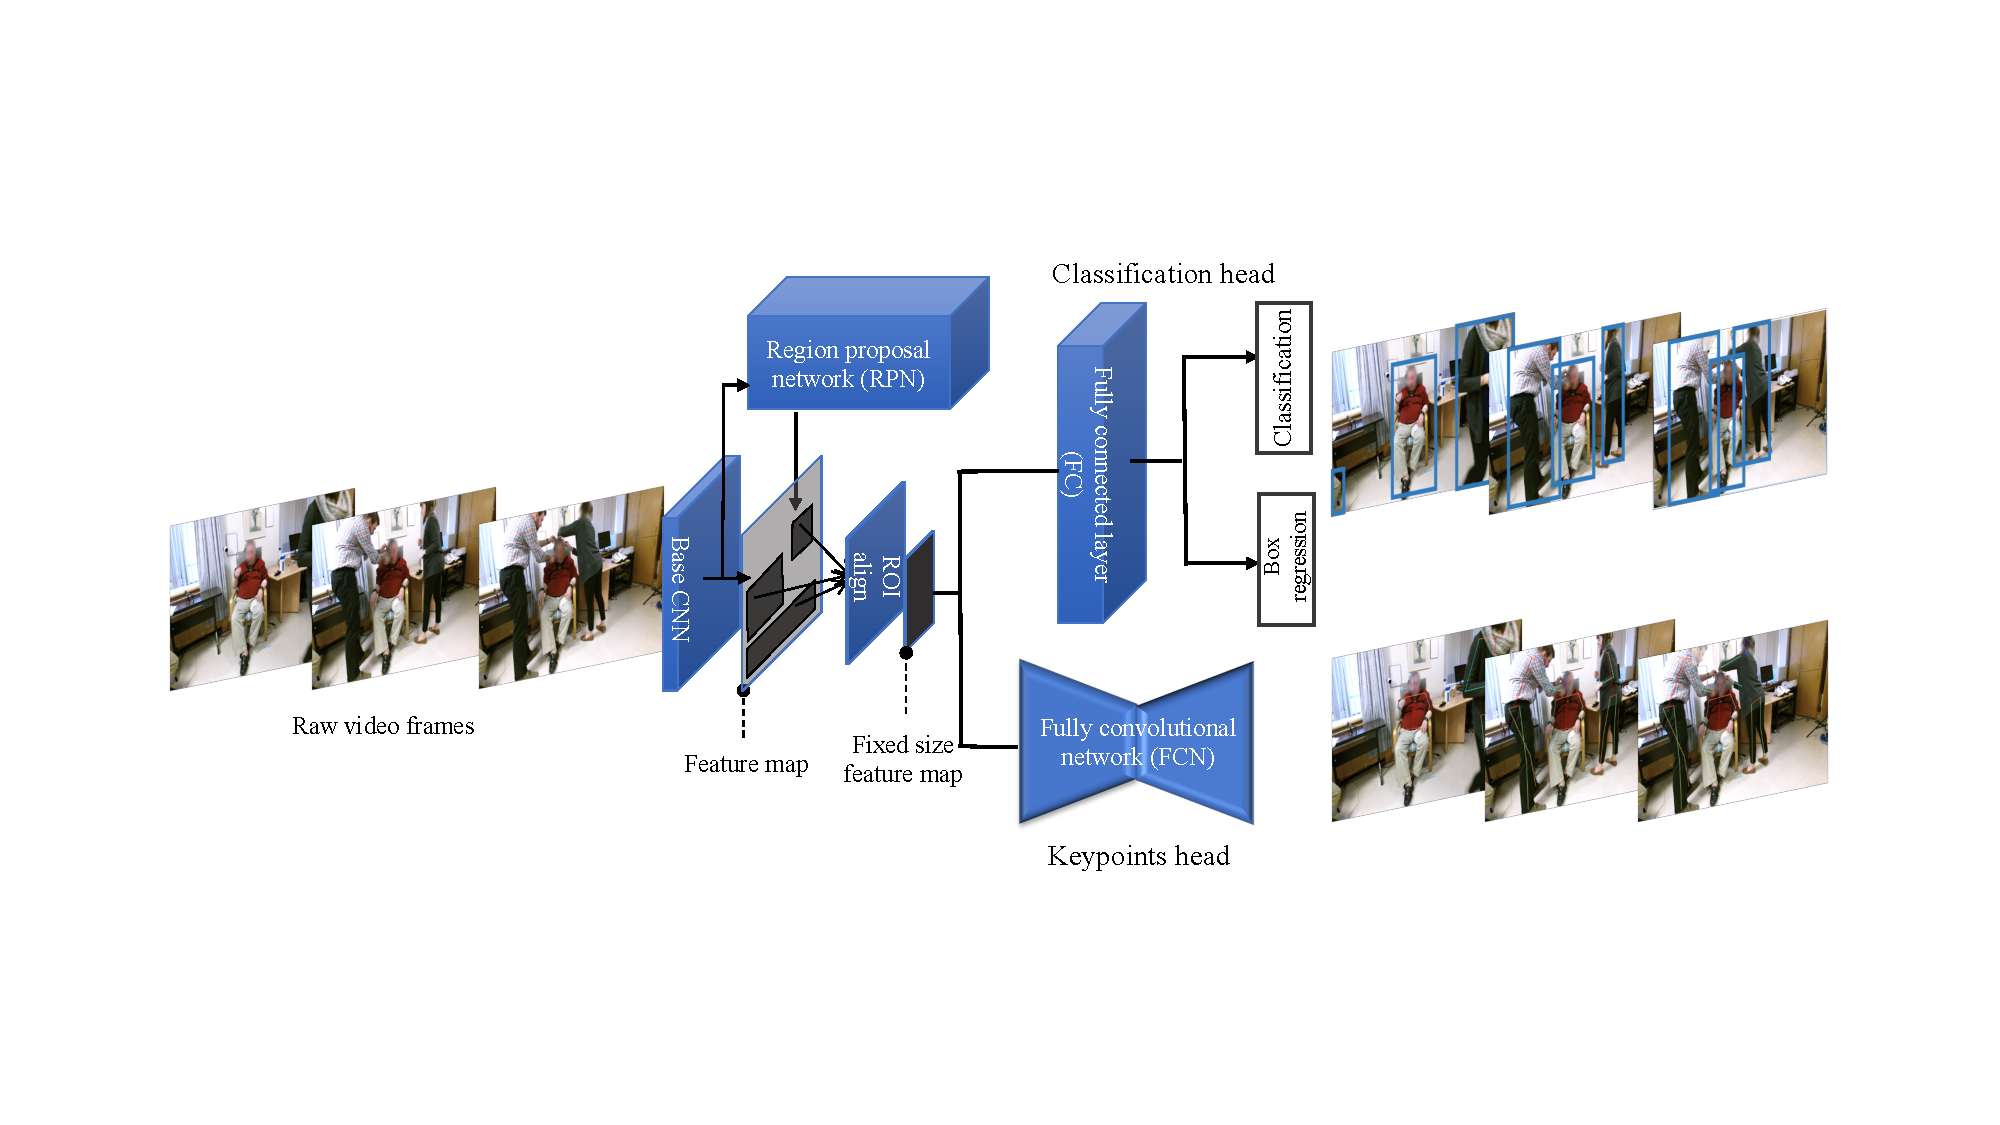
\includegraphics[width=0.9\textwidth, trim=1.1in 1.6in 1.1in 1.6in, clip=true]{Figures/PoseNet.pdf}
    \caption{Architecture of the pose estimation network. Each video frame is fed separately to the base network (ResNet 101) for feature extraction. A region proposal network is applied on the output feature map to find the areas with the highest objectness probability. The fixed size features for proposed regions are then given to the classification and pose estimation heads to find the human bounding boxes and their corresponding keypoints.}
    \label{fig:Pose}
    \vspace{-.1in}
\end{figure*}
}
%====================================
\newcommand{\Tracking}{
\begin{figure*}[t]
    \centering
    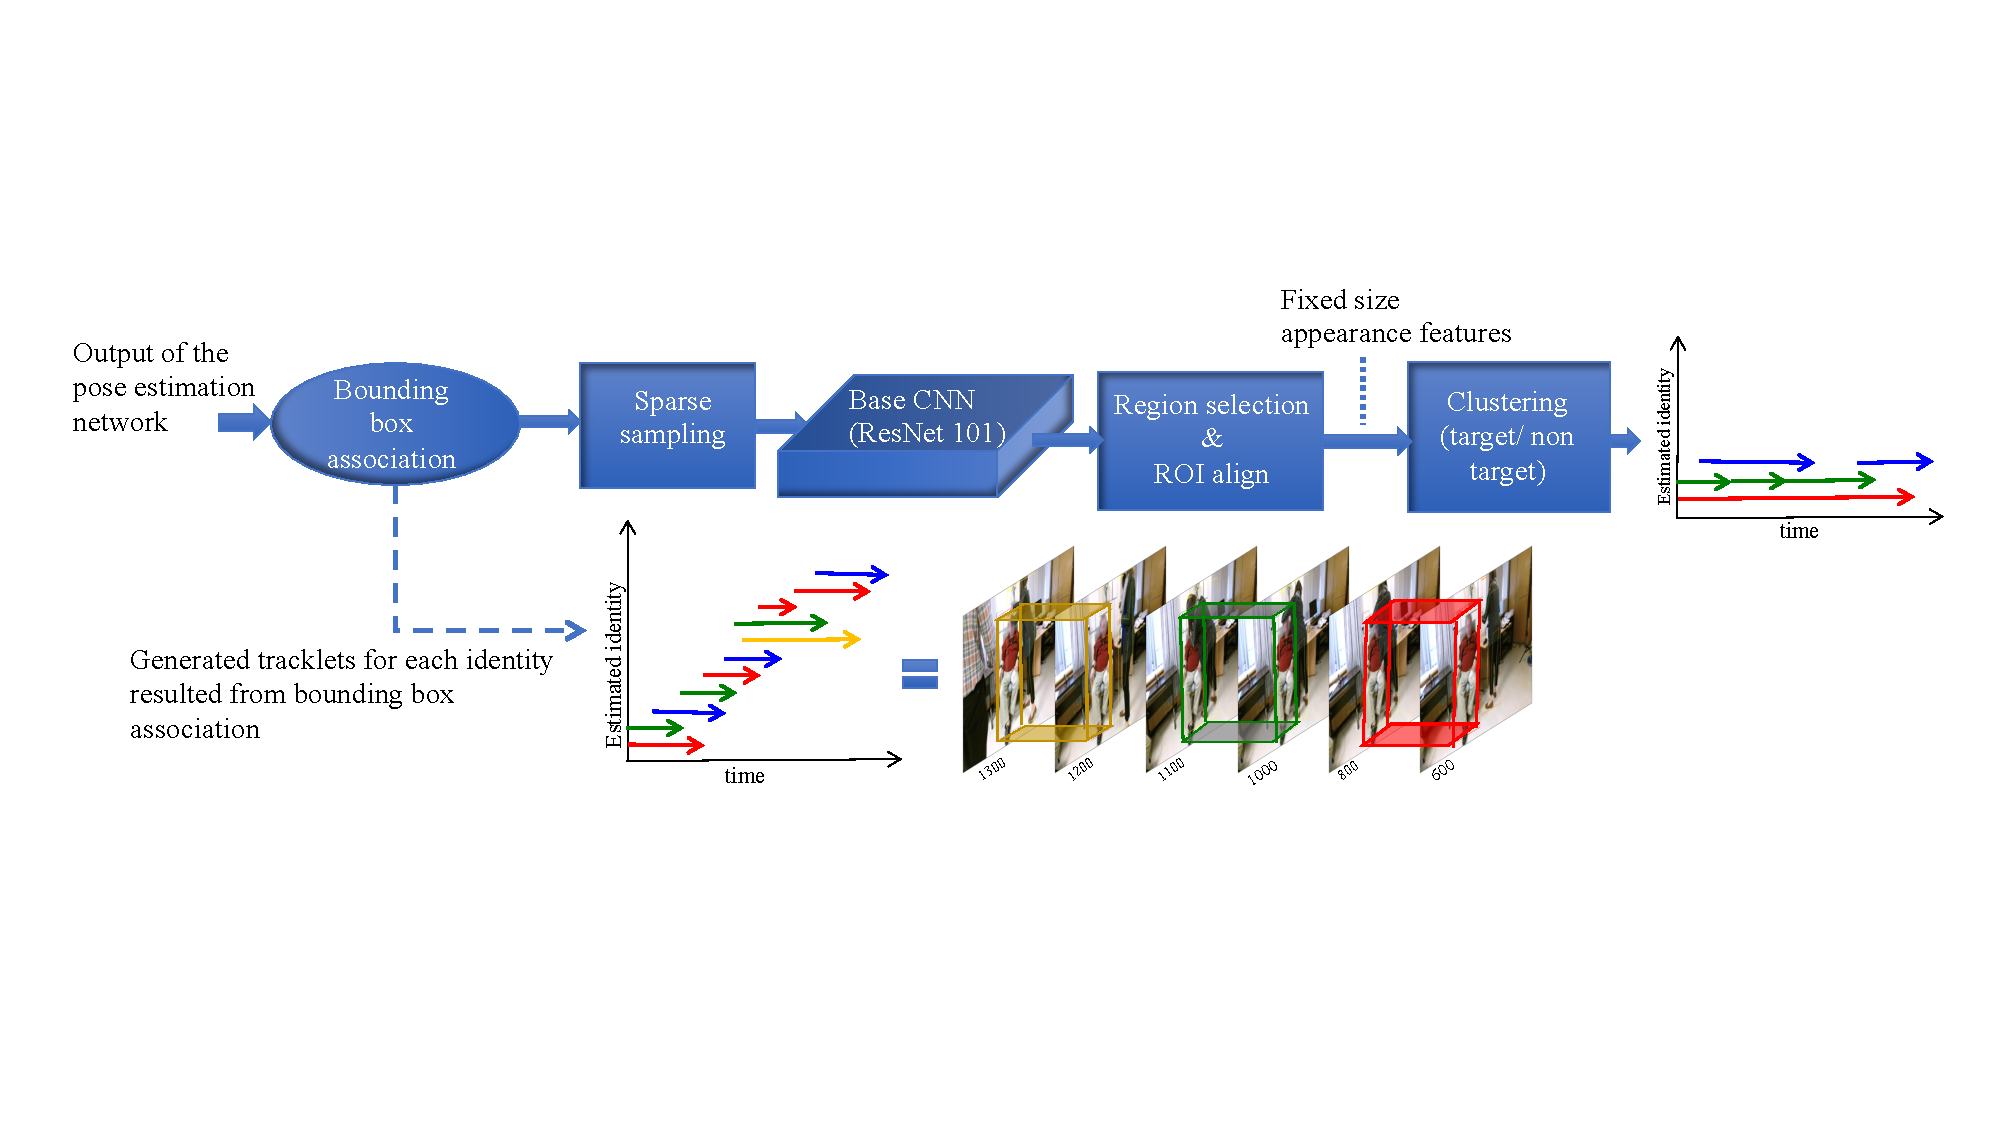
\includegraphics[width=0.9\textwidth, trim=0.1in 2.0in 0.1in 1.8in, clip=true]{Figures/Tracking.pdf}
    \caption{Hierarchical pose tracking using temporal and appearance features. Tracking starts by associating detected bounding boxes in each pair of consecutive frames using the intersection over union metric. Output of this step is a number of different tracklets for each identity. At the next step generated tracklets are pruned based on their length, and pose estimation confidence followed by sparse sampling. Finally, generated tracklets which belong to the target identity are merged according to their appearance similarity to create the endpoint track for the target human actor (best viewed in color).}
    \label{fig:Tracking}
    \vspace{-.1in}
\end{figure*}
}
%=====================================
\newcommand{\ActionNet}{
\begin{figure}[t]
    \centering
    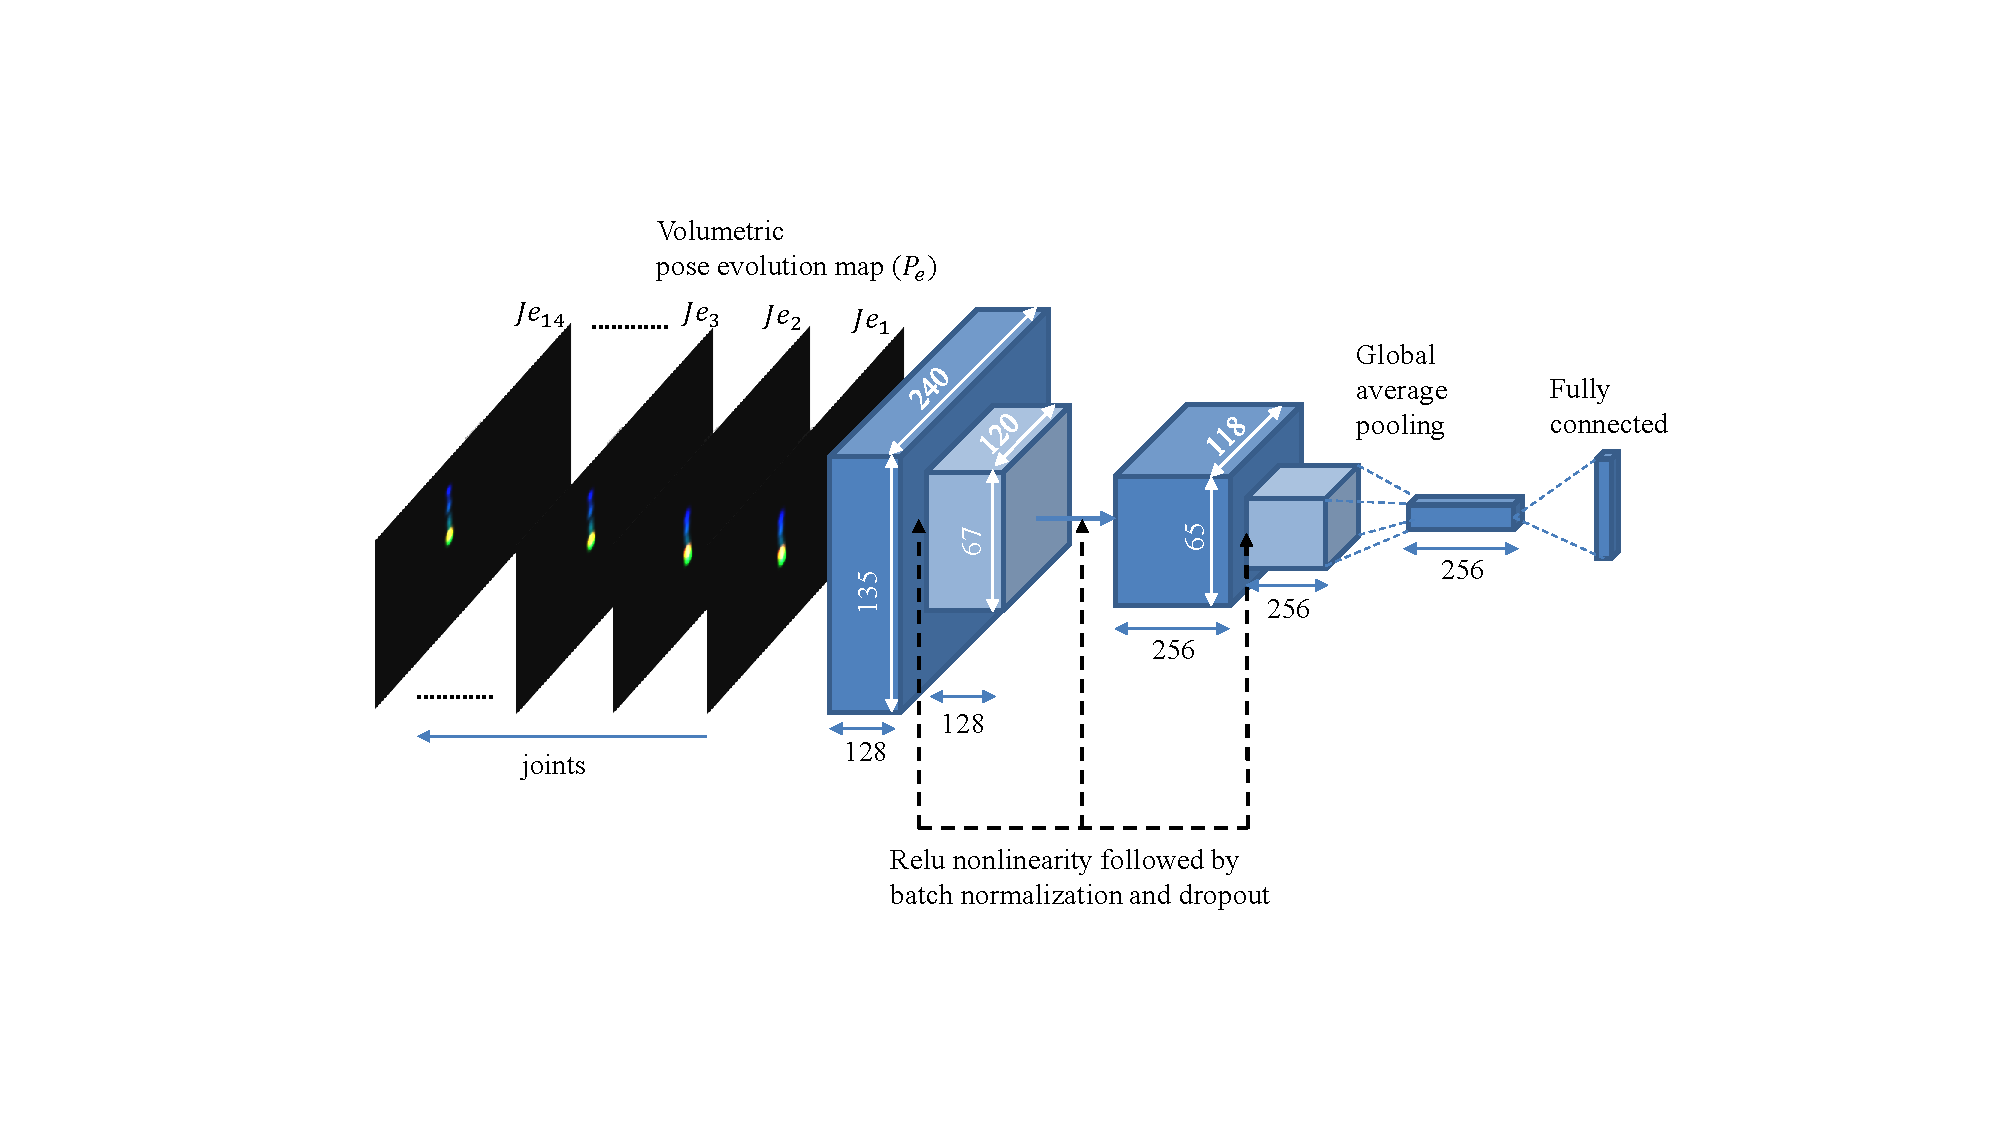
\includegraphics[width=0.5\textwidth, trim=2.1in 1.0in 2.1in 1.0in, clip=true]{Figures/ActionNet.pdf}
    \caption{Architecture of the action classification network. This network takes the volumetric pose evolution map of the target human actor from a video clip as the input and classifies occurrence of an action in the video into one of the five predefined actions (best viewed in color).}
    \label{fig:ActionNet}
    \vspace{-.1in}
\end{figure}
}
%=============================
\newcommand{\ColorCode}{
\begin{figure}[b]
    \centering
    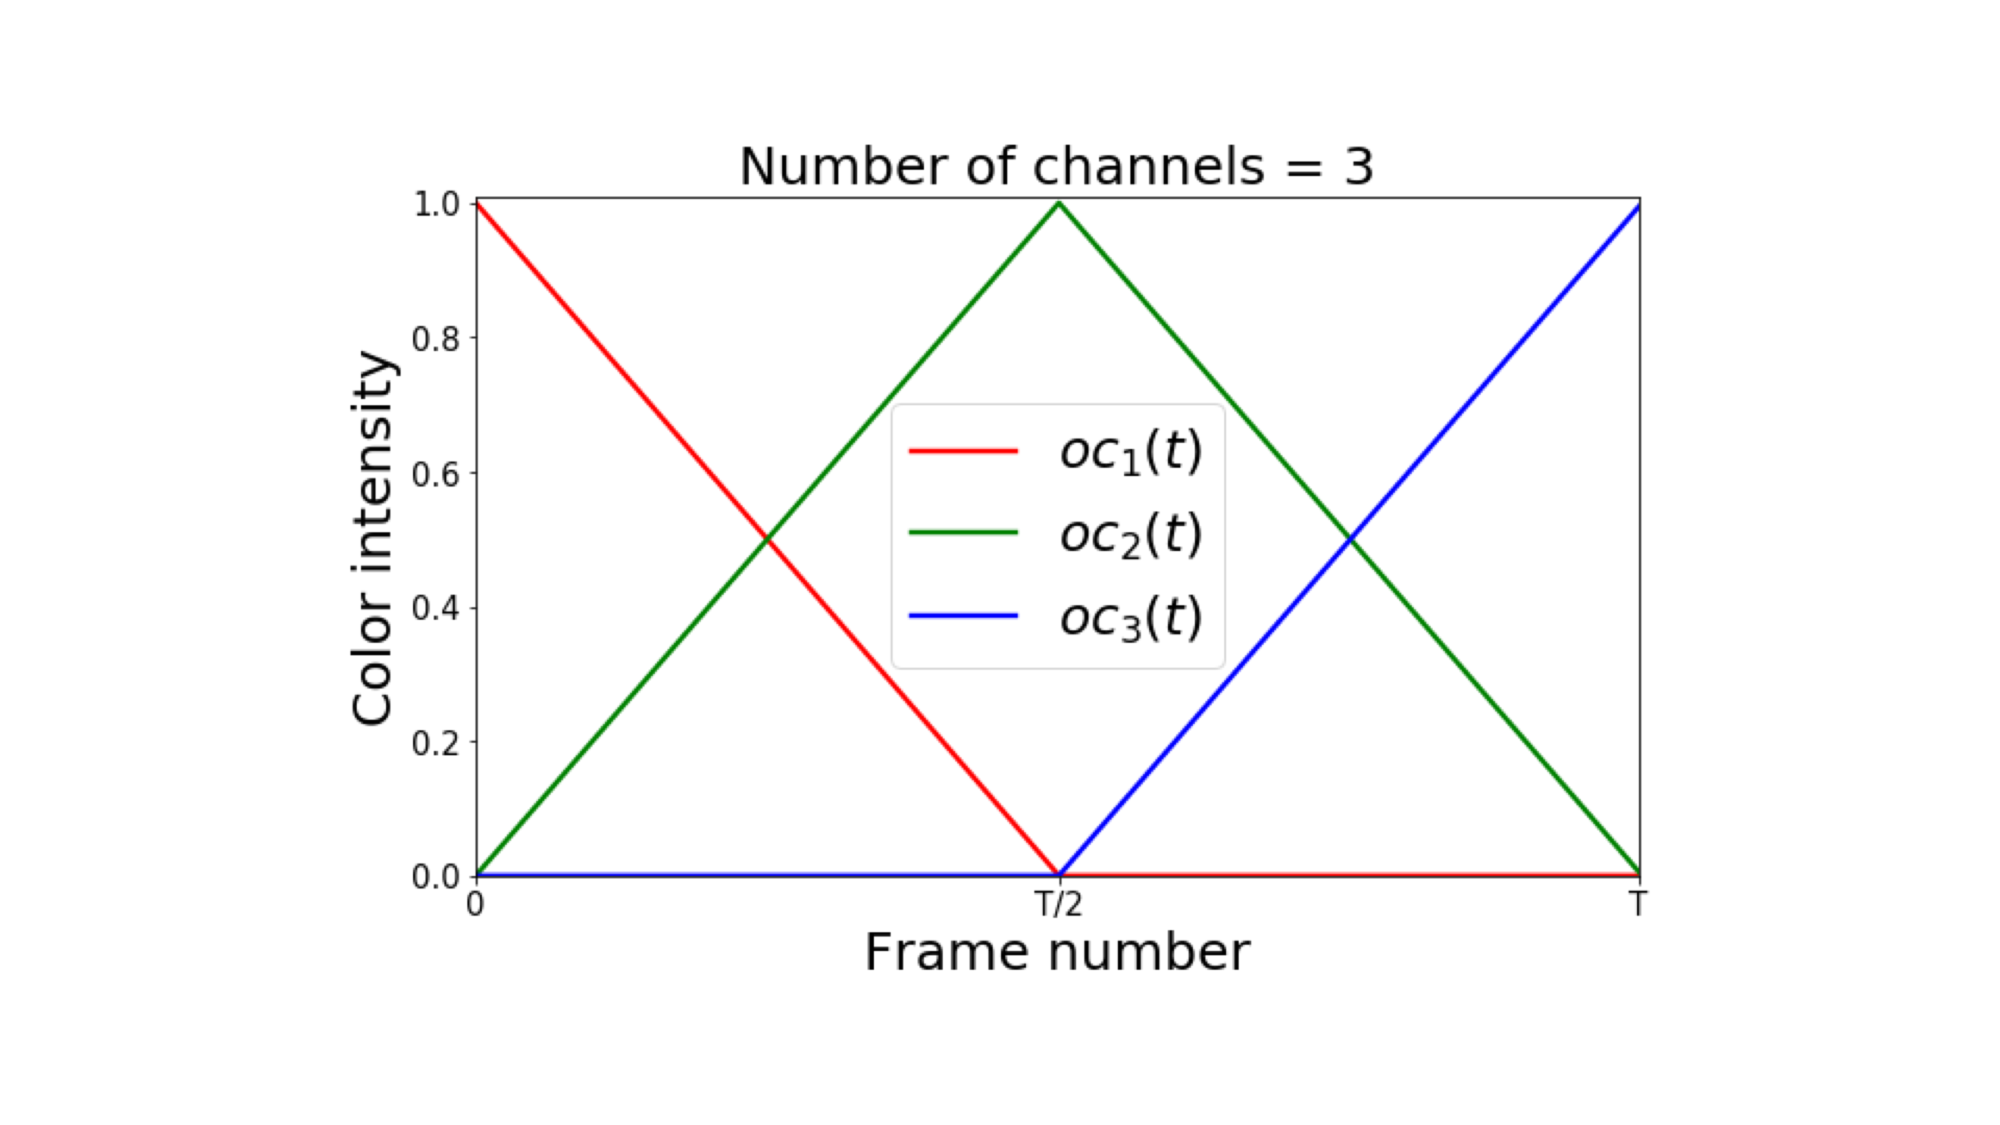
\includegraphics[width=0.27\textwidth, trim=1.9in 0.9in 1.9in 0.9in, clip=true]{Figures/ColorCode.pdf}
    \caption{Demonstration of the time encoded colorization method utilized for creating body pose motion map representation. $oc_1(t)$, $oc_2(t)$, and $oc_3(t)$ show the time encoding function for each color channel.}
    \label{fig:ColorCode}
    \vspace{-.1in}
\end{figure}
}
%===============================
\newcommand{\peseEvolution}{
\begin{figure}[t]
    \centering
    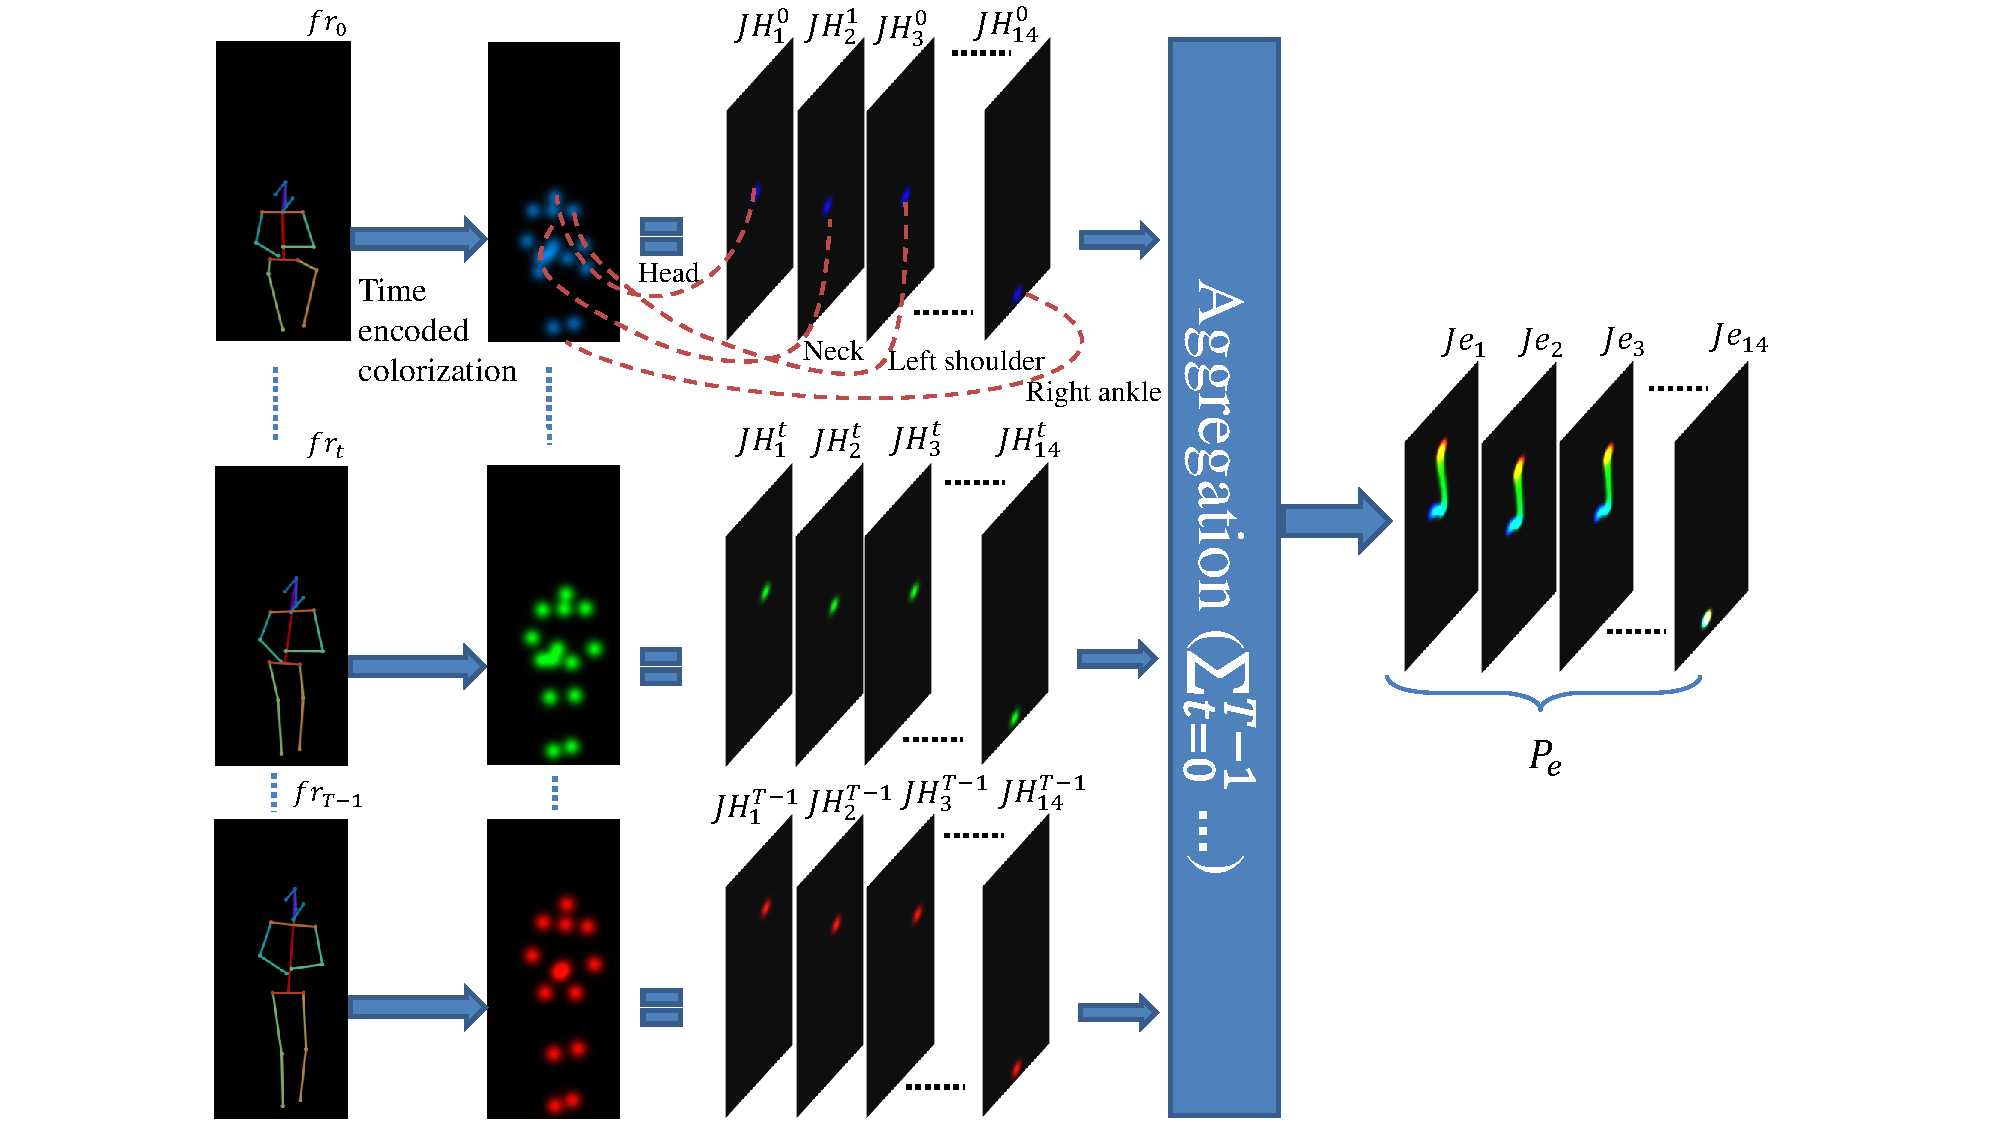
\includegraphics[width=0.5\textwidth, trim=1.0in 0.0in 1.0in 0.0in, clip=true]{Figures/poseEvolution.pdf}
    \caption{Illustration of the pose evolution feature representation in \figref{Method} for the sit-to-stand task. Given the estimated keypoints of the target human actor from preceding stages in the first column, colorized joint heatmaps in the second column are generated using the time encoding function represented in \figref{ColorCode}. The final pose evolution representation is generated by aggregating and normalizing the colorized joint heatmaps in time (best viewed in color).}
    \label{fig:poseEvolution}
%    \vspace{-.1in}
\end{figure}
}
%===============================
\newcommand{\Cmat}{
\begin{figure}[t]
    \centering
    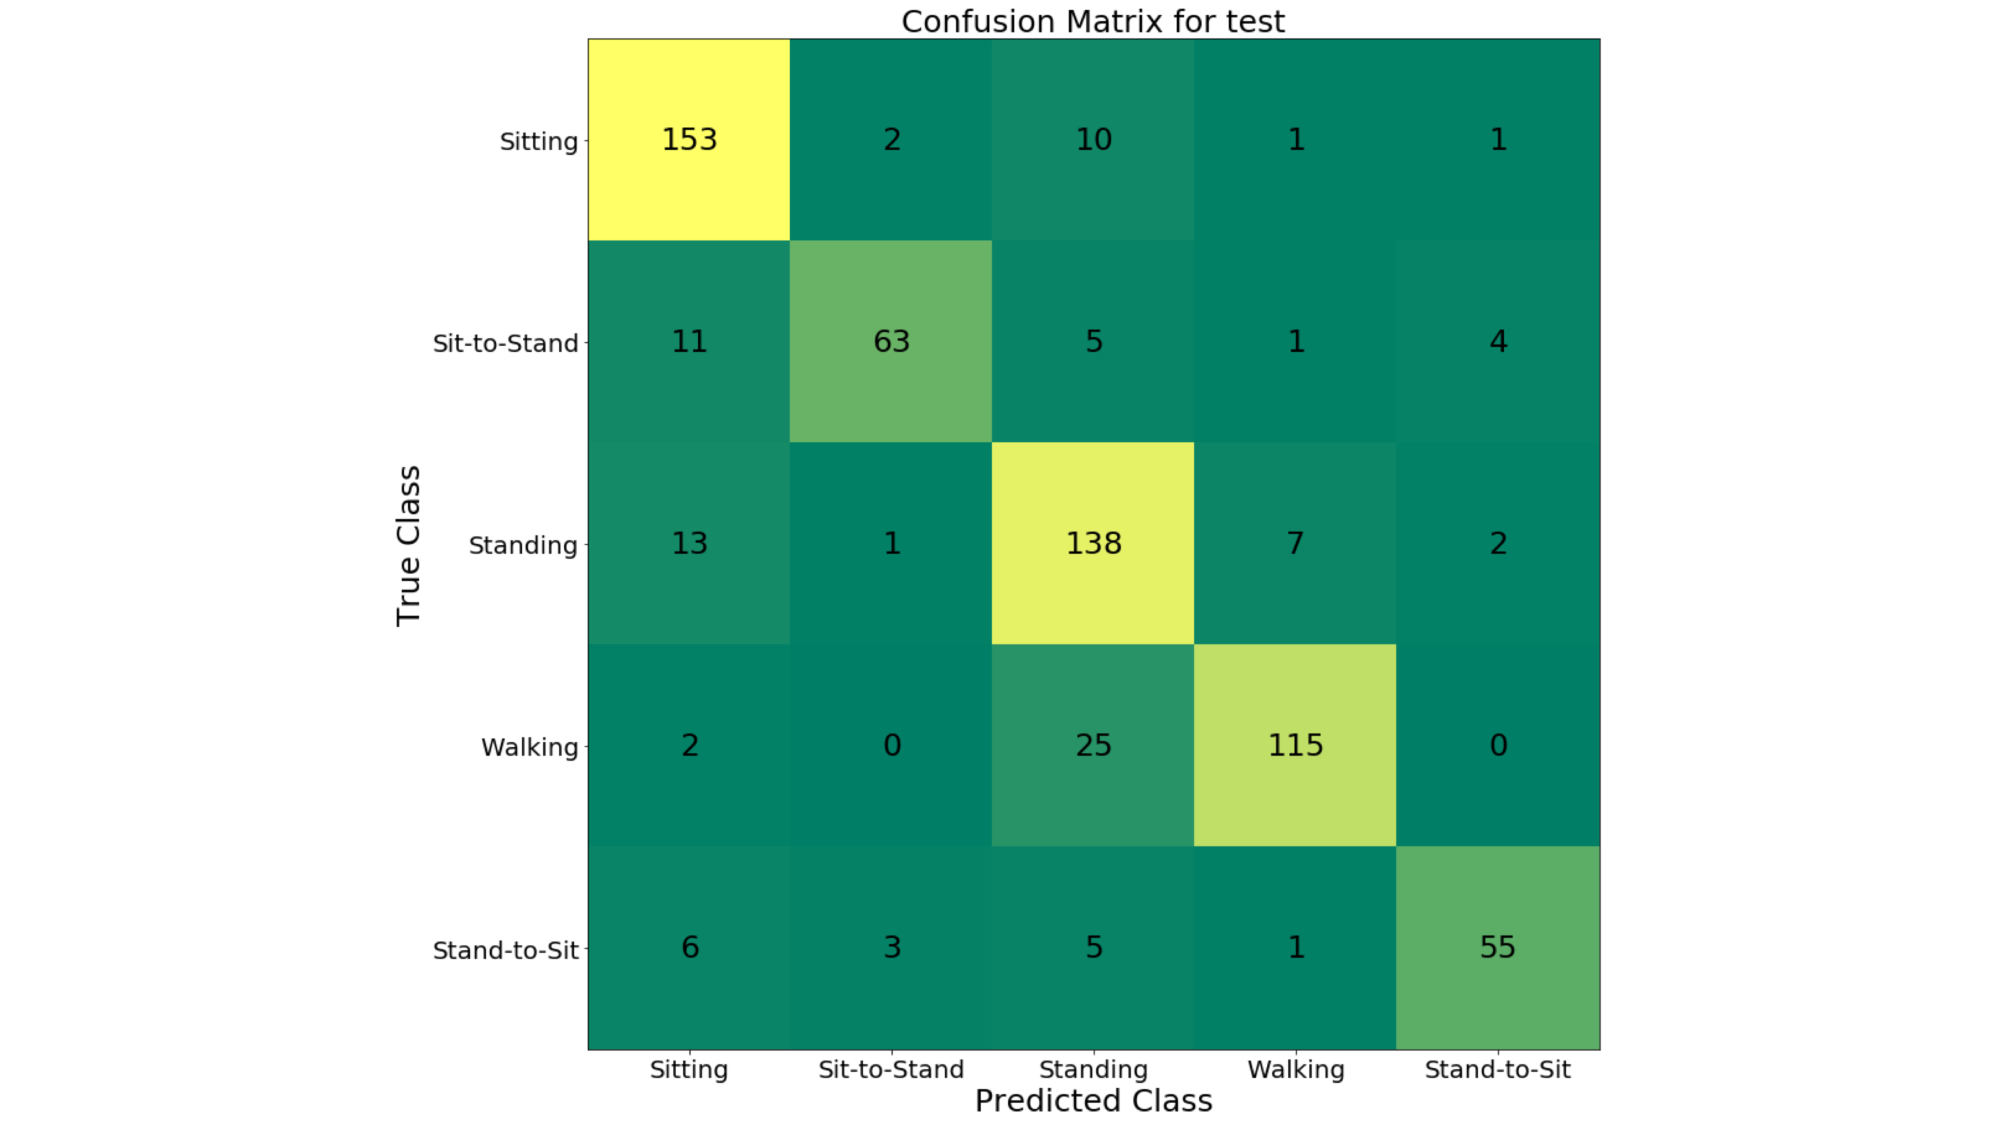
\includegraphics[width=0.35\textwidth, trim=2.5in 0.0in 2.5in 0.0in, clip=true]{Figures/Cmat.pdf}
    \caption{Confusion matrix of the action recognition network evaluated on the test dataset.}
    \label{fig:Cmat}
    \vspace{-.1in}
\end{figure}
}
%=================================
\newcommand{\dataDist}{
\begin{figure}[t]
    \centering
    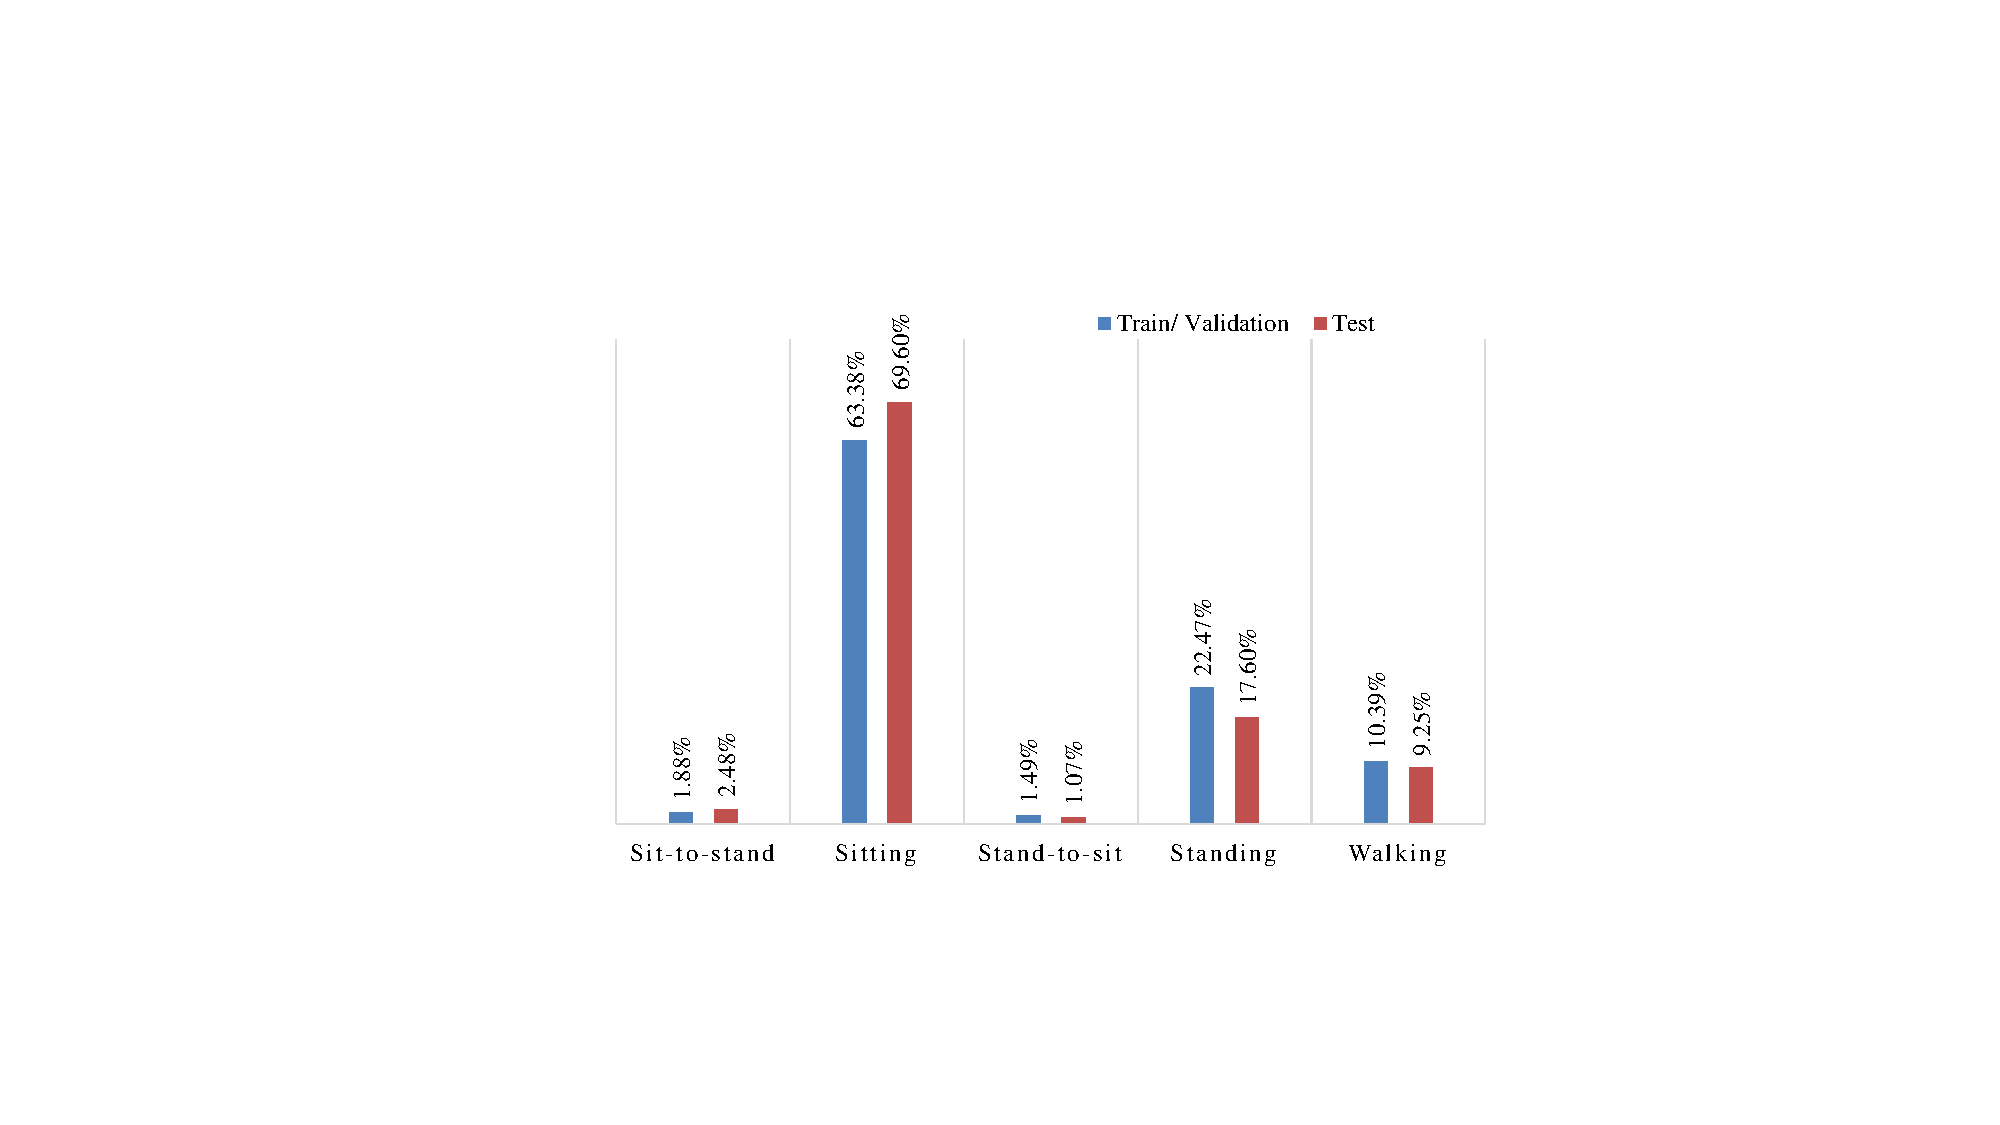
\includegraphics[width=0.4\textwidth, trim=4.1in 1.7in 3.7in 1.8in, clip=true]{Figures/DataDistribution.pdf}
    \caption{Distribution of the action clips based on the type of the actions for test and train/validation datasets. The distribution of the original set of action clips is highly imbalanced. }
    \label{fig:dataDist}
    \vspace{-.1in}
\end{figure}
}
%=================================
\newcommand{\taxonomy}{
\begin{figure}[t]
    \centering
    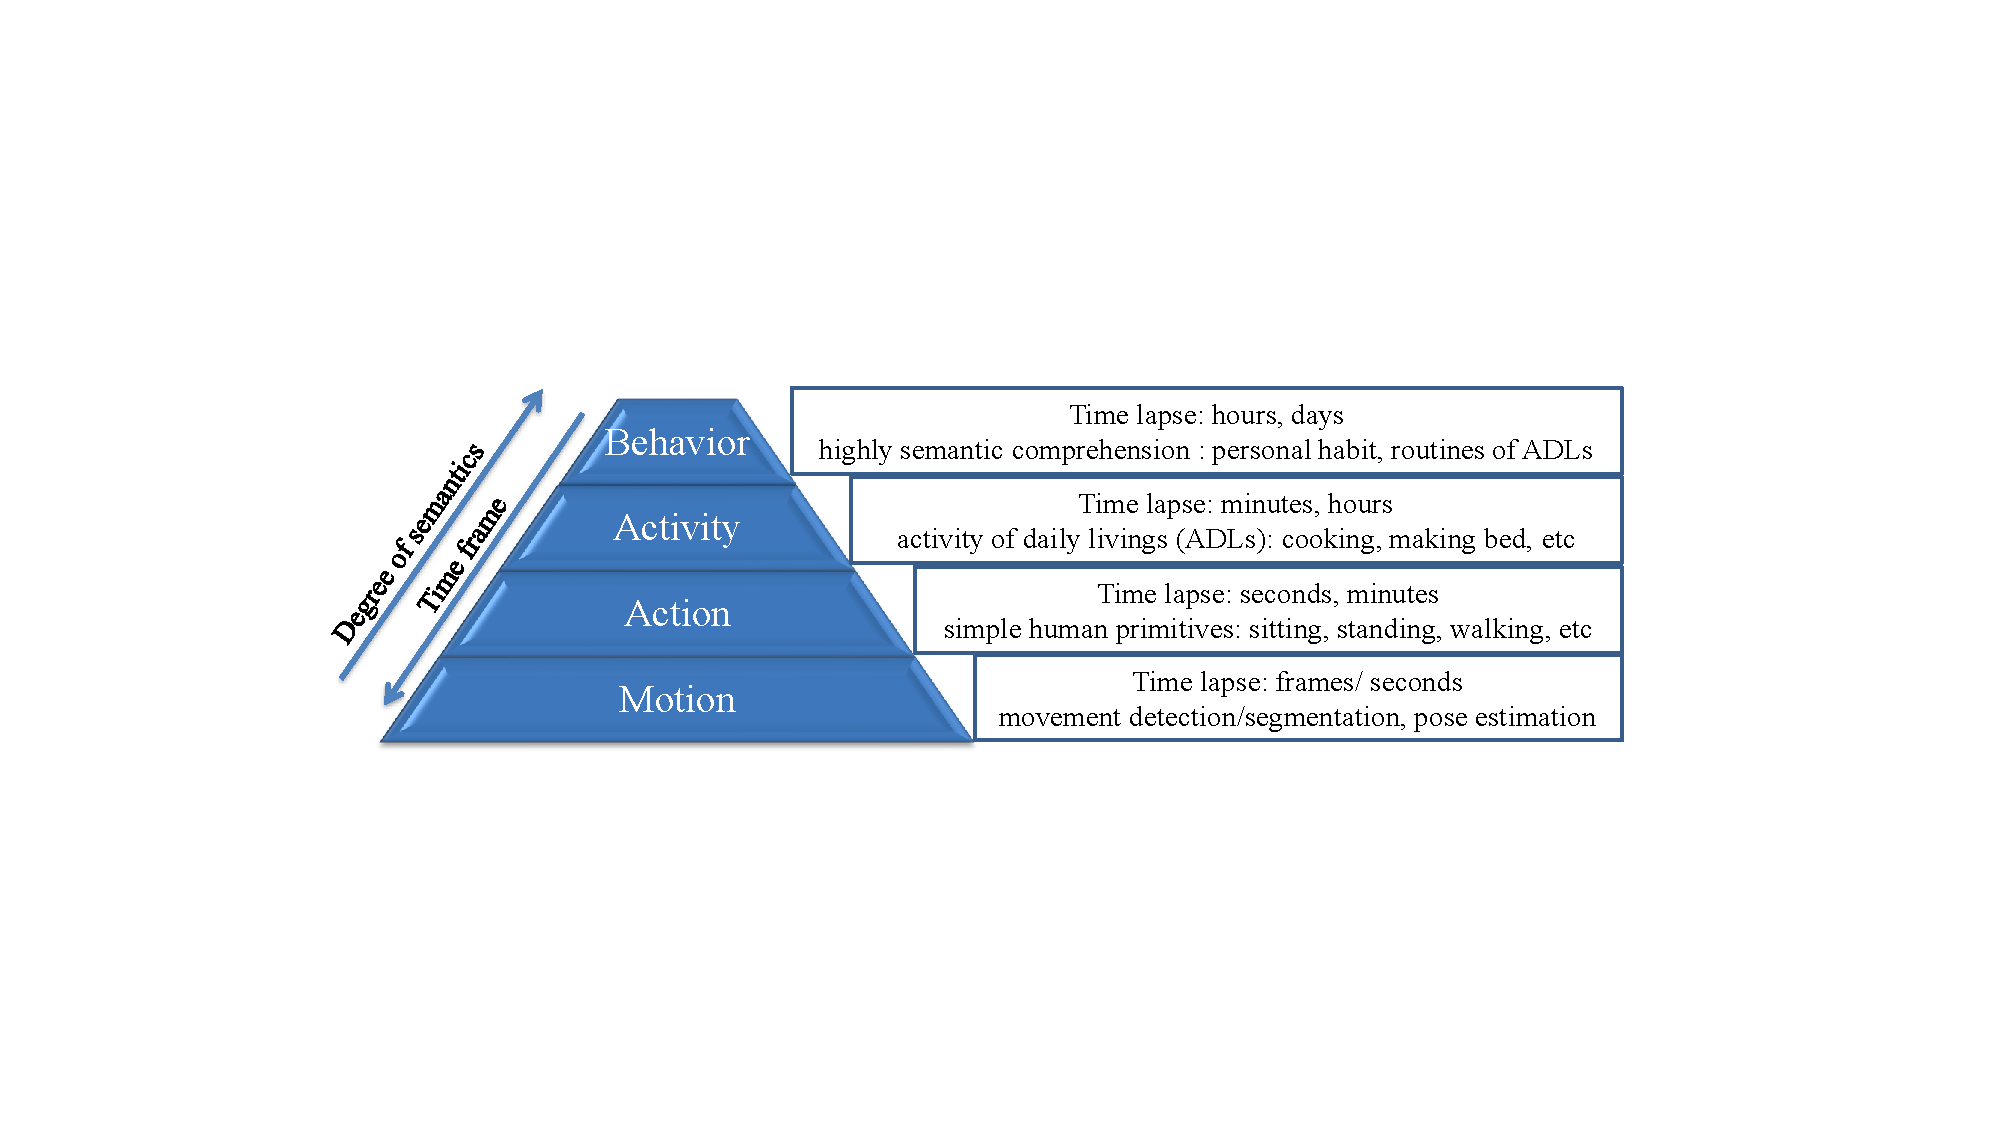
\includegraphics[width=0.5\textwidth, trim=2.2in 2.3in 2.2in 2.3in, clip=true]{Figures/Taxonomy.pdf}
    \caption{Taxonomy of human behaviors with different levels of semantics and complexity. Recognition of each level requires most of the underlying tasks to be recognized \cite{chaaraoui2012review}. }
    \label{fig:taxonomy}
    \vspace{-.1in}
\end{figure}
}

%================================
\newcommand{\chStat}{
\begin{figure}[t]
    \centering
    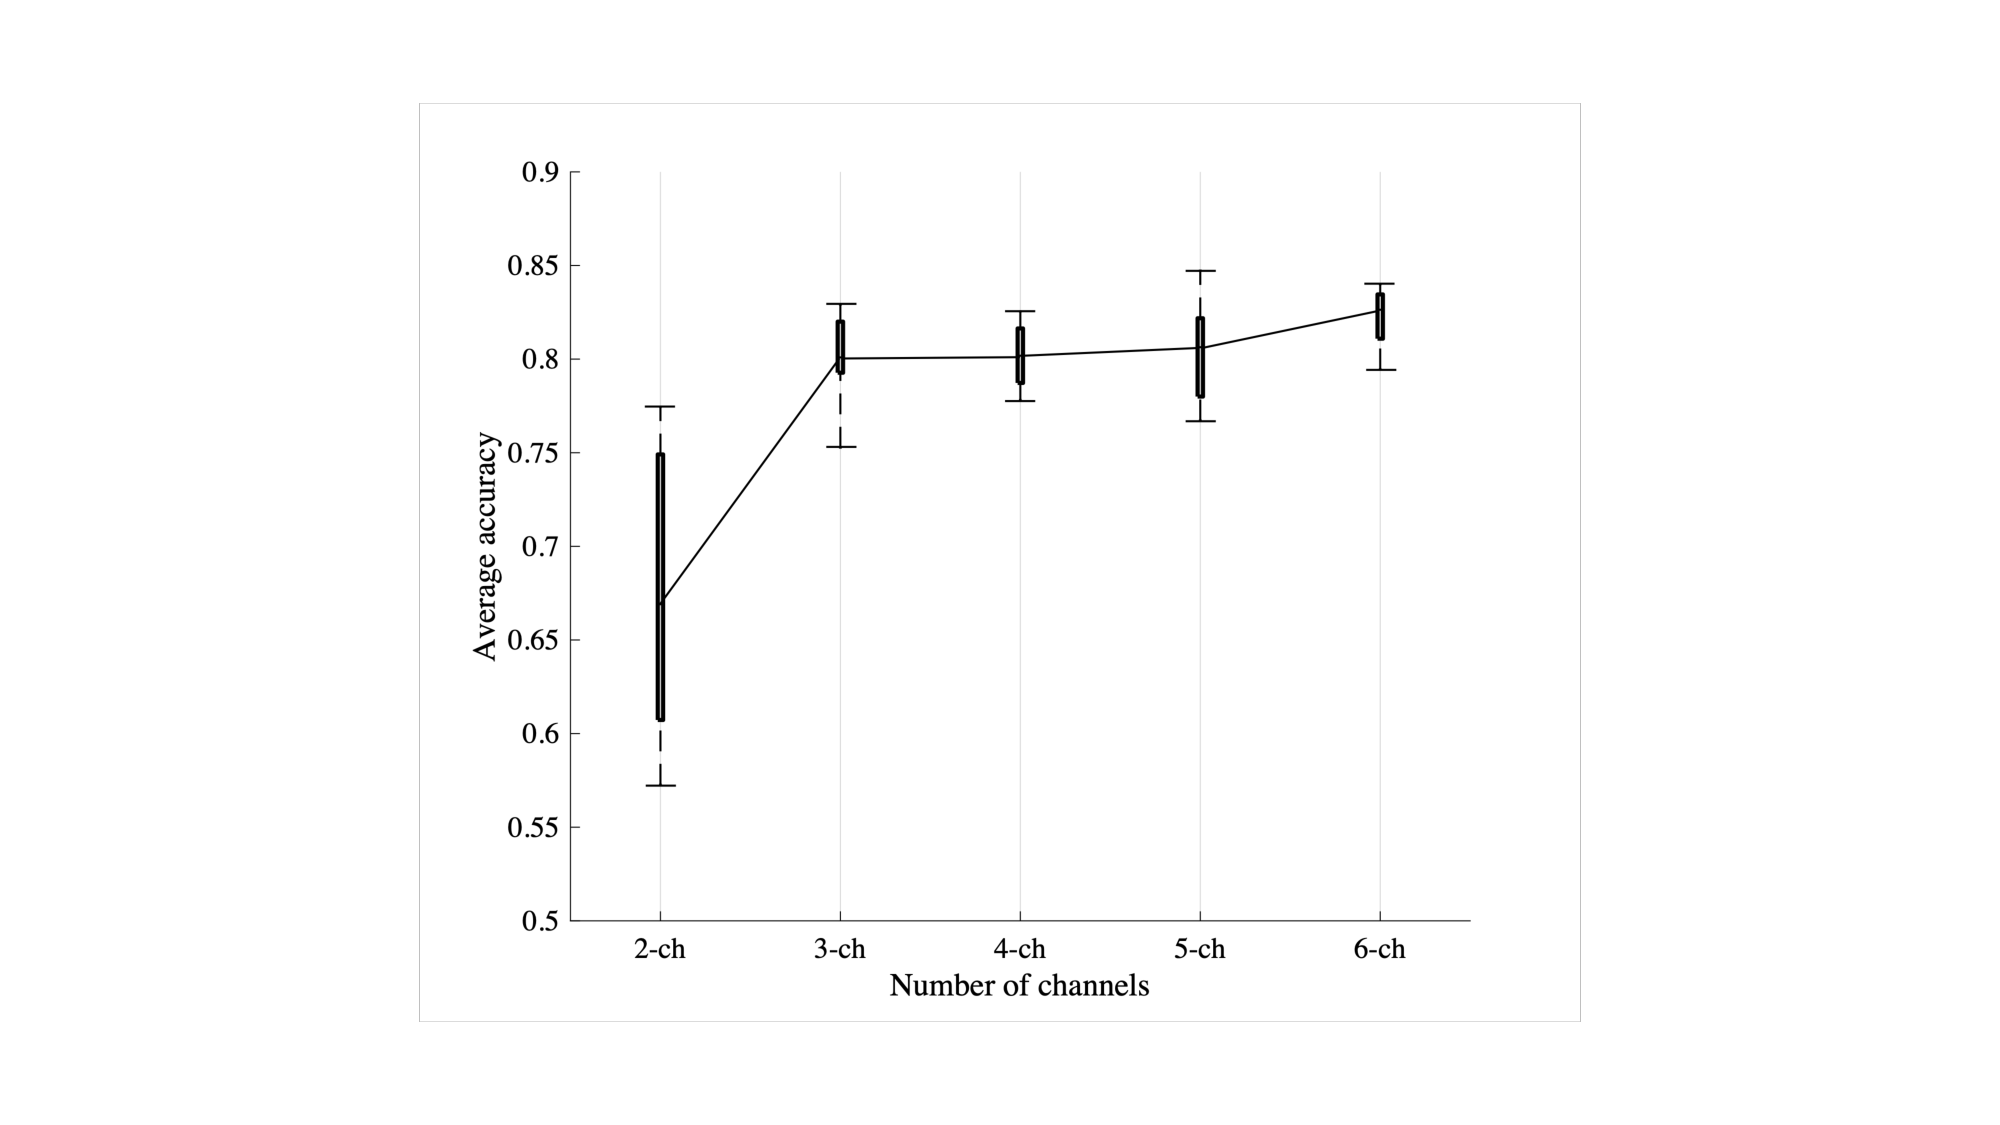
\includegraphics[width=0.35\textwidth, trim=2.7in 0.7in 2.7in 1.0in, clip=true]{Figures/chStat.pdf}
    \caption{Average classification accuracy with respect to the number of channels of input pose evolution representations.}
    \label{fig:chStat}
    \vspace{-.1in}
\end{figure}
}

%====================================

\newcommand{\missclass}{
\begin{figure}[t]
 \centering
  \subfloat[][Standing]{\label{fig:stand}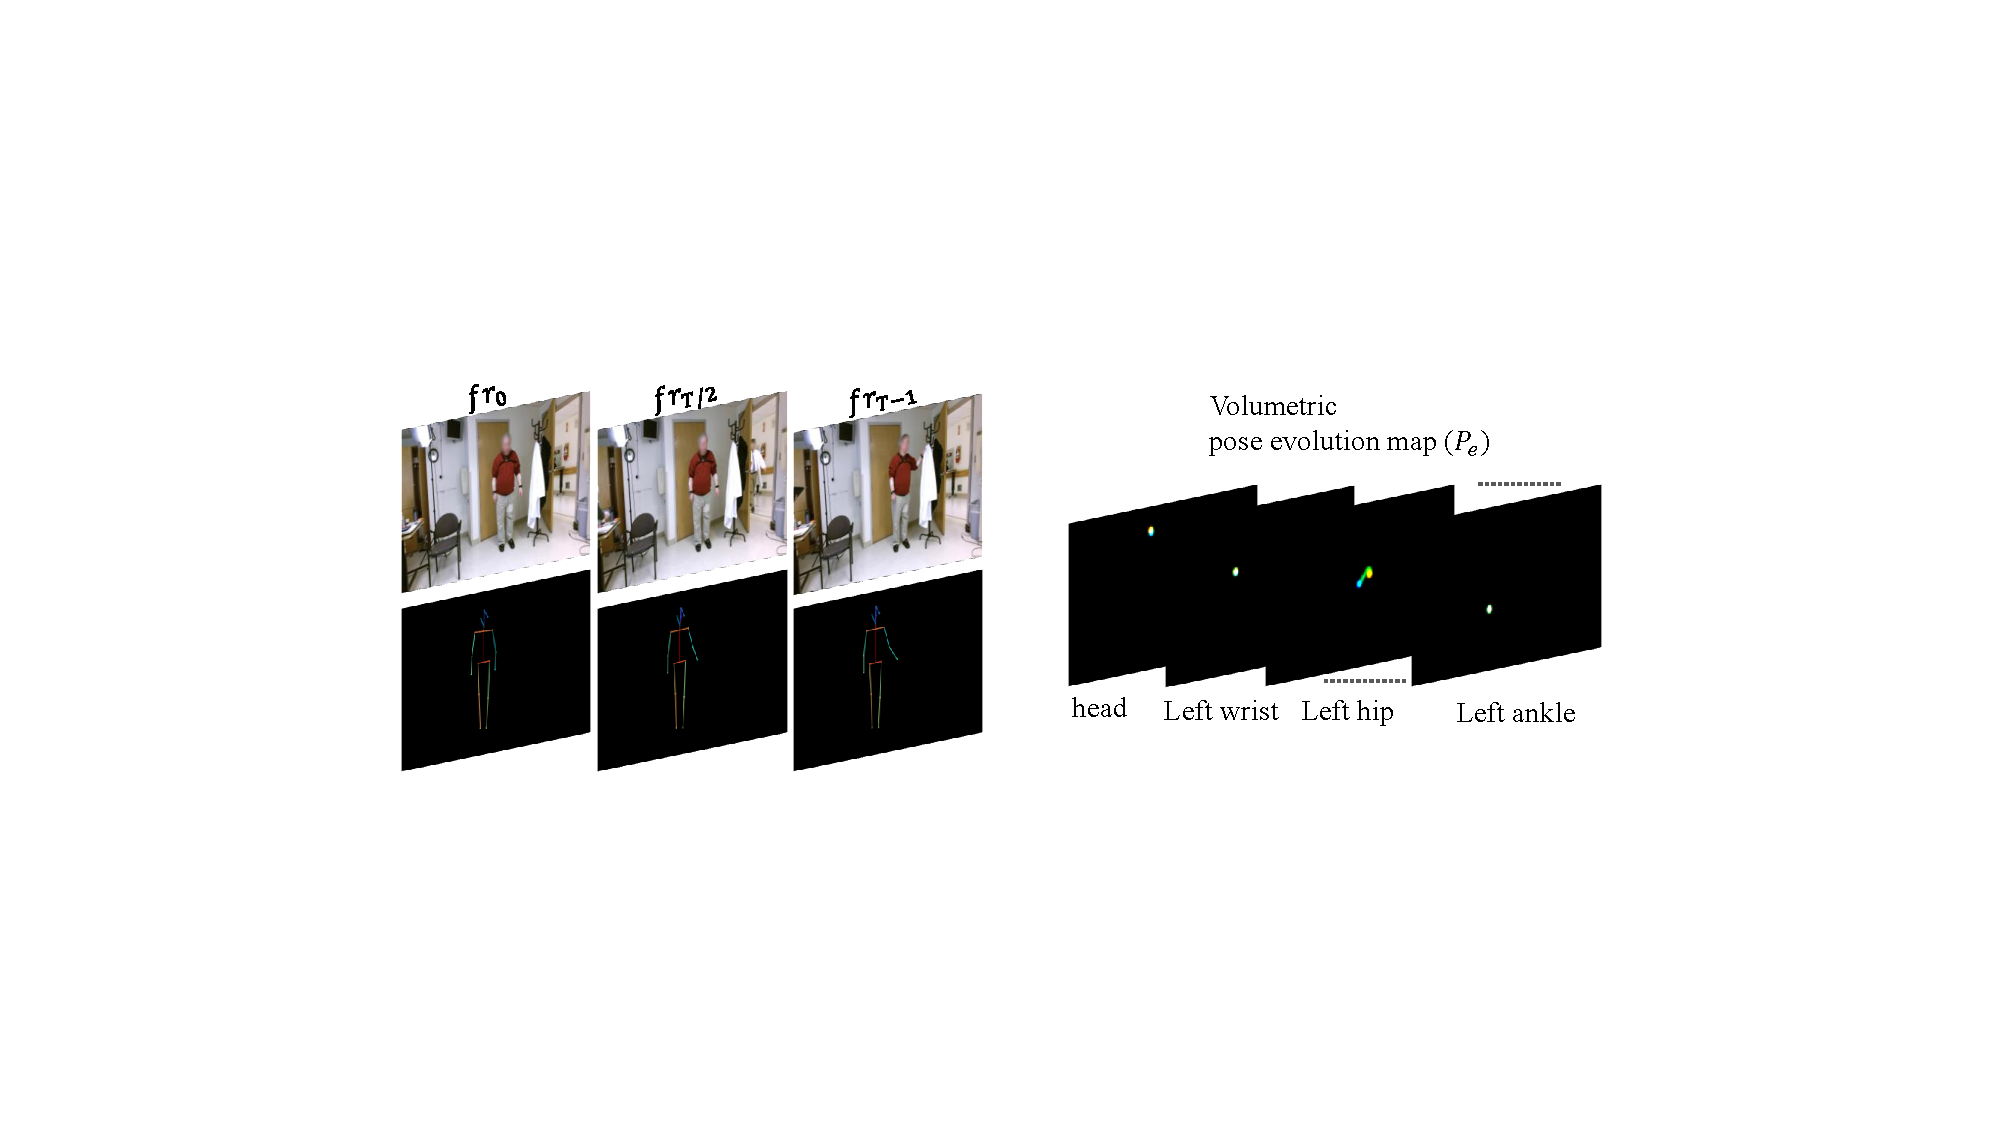
\includegraphics[width=0.5\textwidth, trim=2.5in 2.35in 2.4in 2.5in, clip=true]{Figures/standing.pdf}}\\
  \vspace{-.06in}
 \subfloat[][Transition from standing to walking]{\label{fig:transit}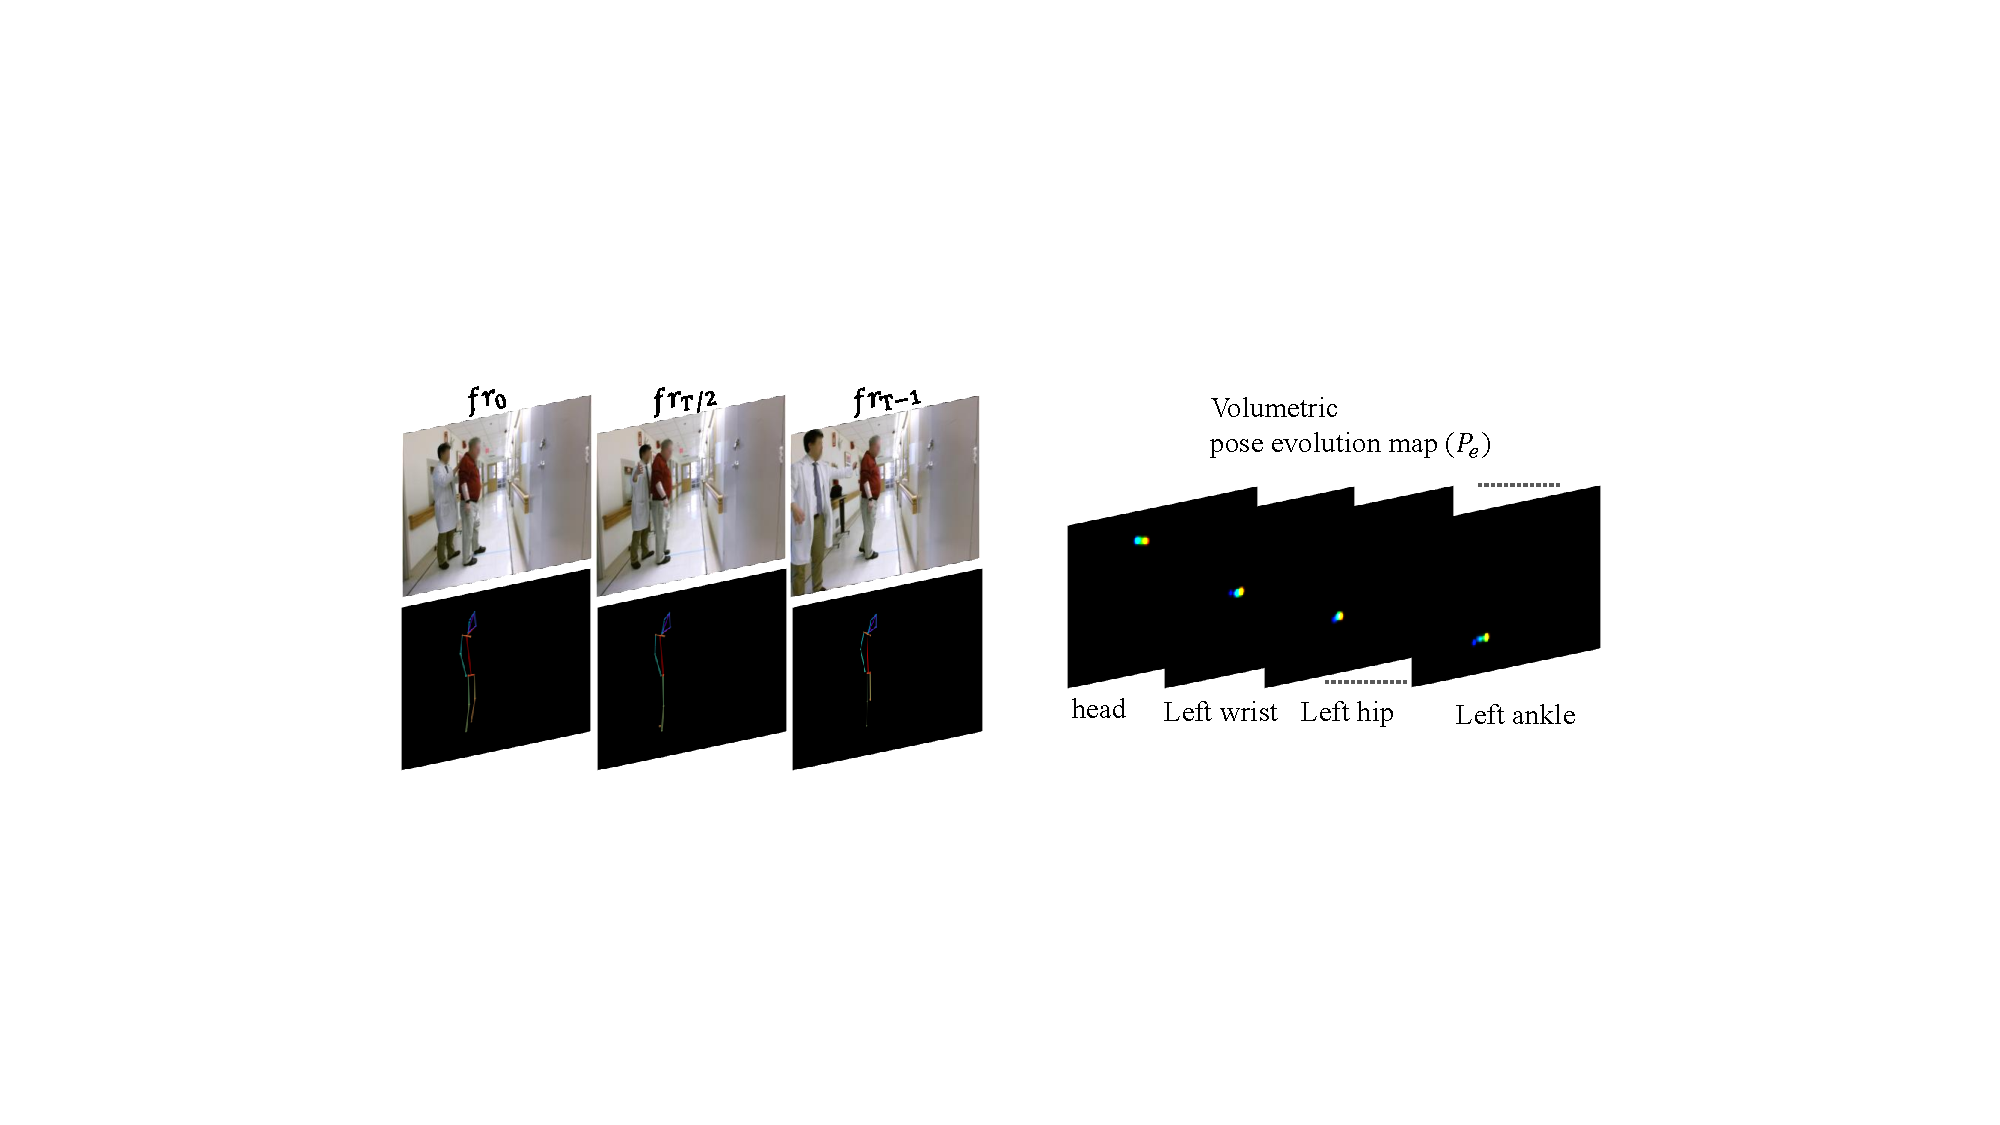
\includegraphics[width=0.5\textwidth, trim=2.5in 2.35in 2.4in 2.5in,
  clip=true]{Figures/transition.pdf}}\\
  \vspace{-.06in}
 \subfloat[][Walking in frontal view]{\label{fig:walk}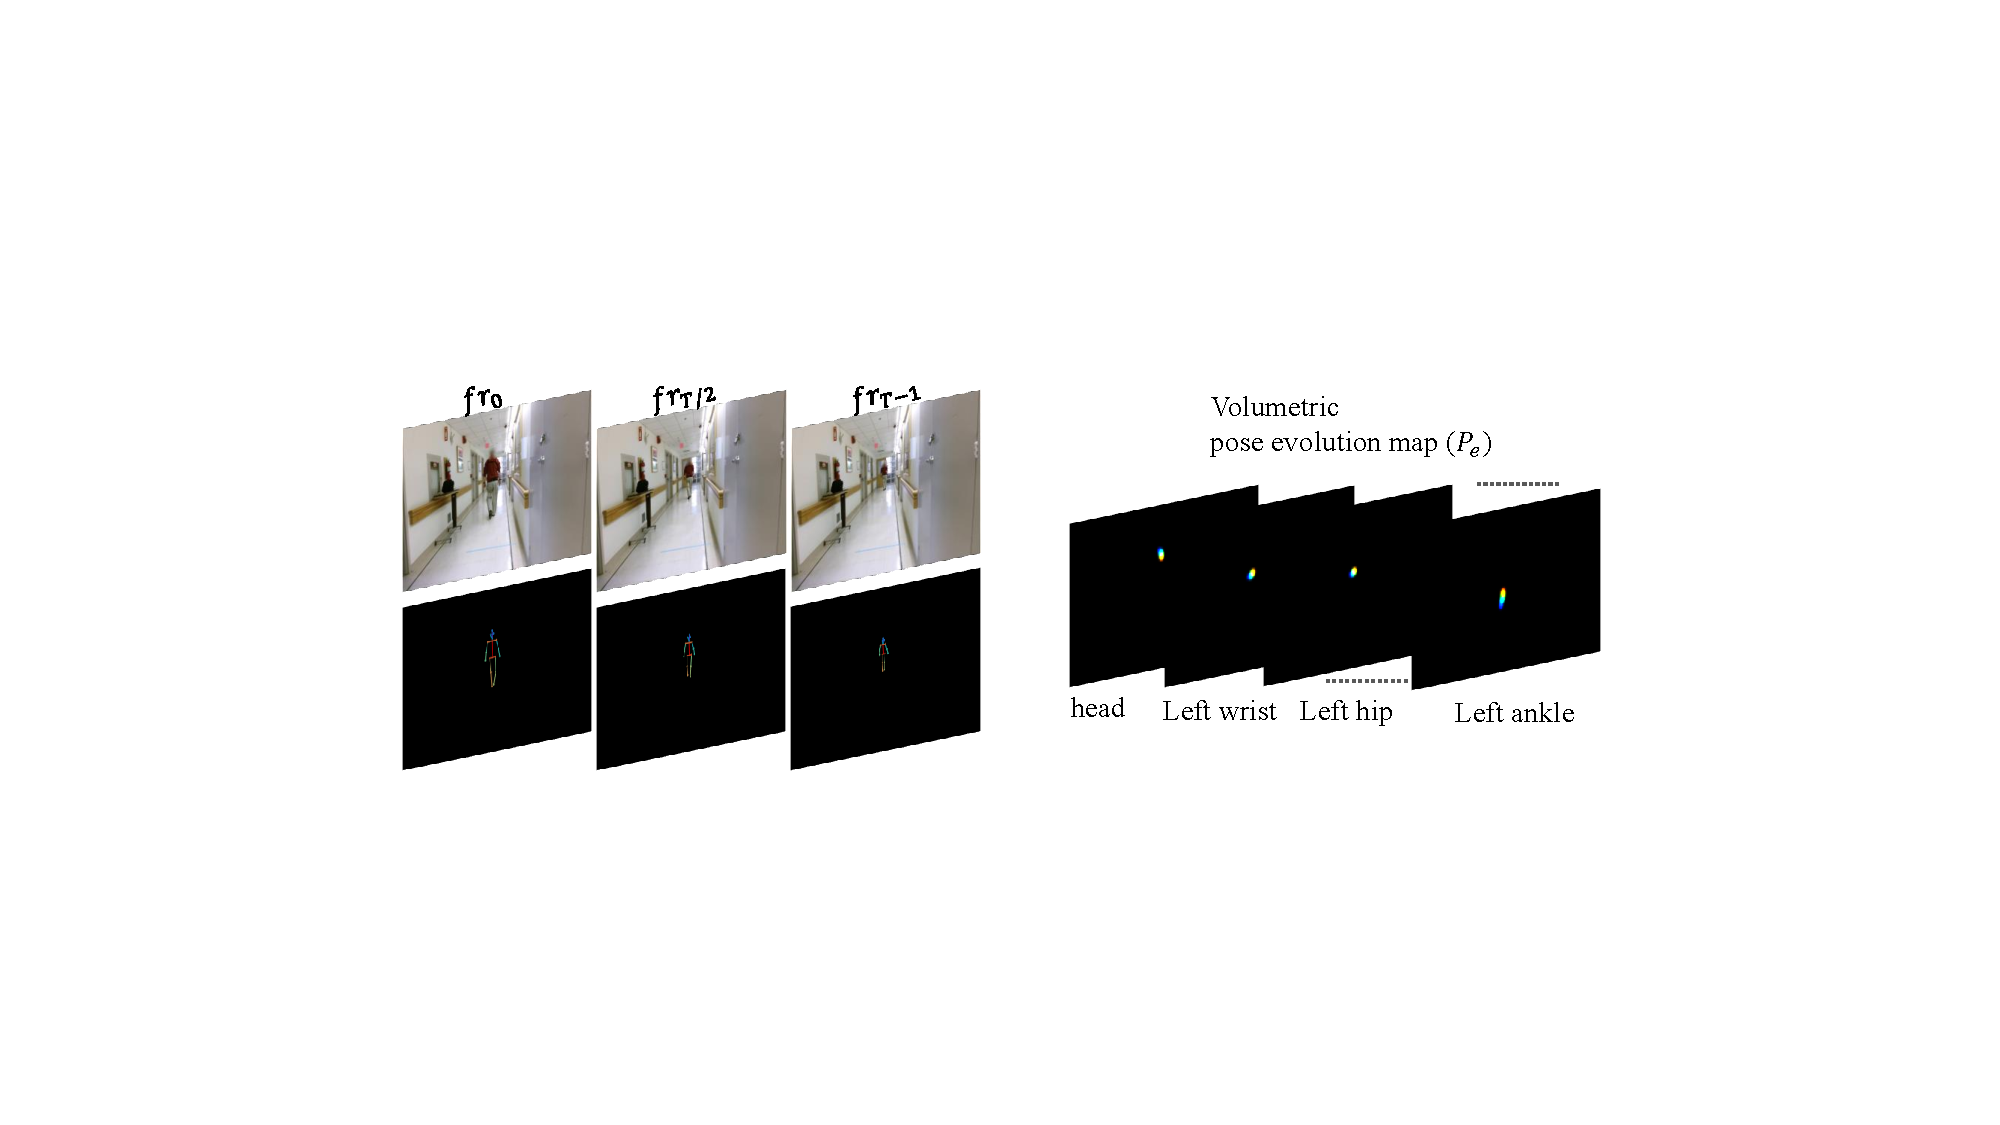
\includegraphics[width=0.5\textwidth,trim=2.5in 2.35in 2.4in 2.5in,
  clip=true]{Figures/walking.pdf}}\\
  \caption{An example of the misclassification of walking as standing. (a), (b), and (c) show the first, middle, and last frame of three action video clips along with the corresponding pose estimations and pose evolution maps. During the manual annotation process (a) was labeled as standing, whereas (b) and (c) were labeled as walking. The action classification network classifies (a) and (b) as standing because they have a very similar pose evolution map (best viewed in color and zoomed in). }
\label{fig:missclass}
\vspace{-.1in}
\end{figure}
}
%=================== Tables
\newcommand{\accuracy}{
\begin{table}[b] 
\scriptsize
\begin{center}
 \begin{tabular}{c|c c c c c c} 
    & Sit & \shortstack{Sit-to-stand} & Stand & Walk &\shortstack{Stand-to-sit}  & \shortstack{Average \\ accuracy} \\ 
  \hline
  Validation & 92.8 & 68.1 & 81.5 & 78.9 & 70.7 & 80.5 \\
  \hline
  Test & 91.6 & 75.0 & 85.7 & 81.0 & 78.6 & 84.0

\end{tabular}
\end{center}
 \caption{\footnotesize Classification accuracy (\%) on the test and validation set.}
\vspace{-.2in}
\label{tbl:accuracy}
\end{table}
}
%%%%%%%%%%%%

% If you comment hyperref and then uncomment it, you should delete
% egpaper.aux before re-running latex.  (Or just hit 'q' on the first latex
% run, let it finish, and you should be clear).
\usepackage[pagebackref=true,breaklinks=true,colorlinks,bookmarks=false]{hyperref}
% correct bad hyphenation here
%\hyphenation{op-tical net-works semi-conduc-tor}


\begin{document}
%
% paper title
% Titles are generally capitalized except for words such as a, an, and, as,
% at, but, by, for, in, nor, of, on, or, the, to and up, which are usually
% not capitalized unless they are the first or last word of the title.
% Linebreaks \\ can be used within to get better formatting as desired.
% Do not put math or special symbols in the title.
\title{Target-Specific Action Classification for Automated Phenotyping of Human Motor Behavior from Video} %Toward AI assisting Health-care}
%
%
% author names and IEEE memberships
% note positions of commas and nonbreaking spaces ( ~ ) LaTeX will not break
% a structure at a ~ so this keeps an author's name from being broken across
% two lines.
% use \thanks{} to gain access to the first footnote area
% a separate \thanks must be used for each paragraph as LaTeX2e's \thanks
% was not built to handle multiple paragraphs
%

\author{Behnaz~Rezaei,~\IEEEmembership{student member},~IEEE,
        Yiorgos~Christakis,
        Bryan~Ho,
        Kevin~Thomas,
        Kelley~Erb,
        Sarah~Ostadabbas,~\IEEEmembership{member},~IEEE,
        and~Shyamal~Patel,~\IEEEmembership{member},~IEEE.% <-this % stops a space
\thanks{B. Rezaei and S. Ostadabbas are with the Augmented Cognition Lab (ACLab) at the Department
of Electrical and Computer Engineering, Northeastern University, Boston,
MA 02115, USA. e-mails: \{brezaei, ostadabbas\}@ece.neu.edu.
B. Ho is with the Neurology Department at Tufts University School of Medicine, Boston, MA 02111, USA. email: bho@tuftsmedicalcenter.org.
K. Thomas is with the Department of Anatomy & Neurobiology at Boston University School of Medicine, Boston, MA 02118, USA. email: kipthoma@bu.edu.
Y. Christakis, Kelley Erb and S. Patel are with the Digital Medicine \& Translational Imaging group at Pfizer, Cambridge, MA 02139, USA. e-mails: \{Yiorgos.Christakis, MichaelKelley.Erb, Shyamal.Patel\}@pfizer.com.
}
}% <-this % stops a space
%\thanks{J. Doe and J. Doe are with Anonymous University.}% <-this % stops a space
%\thanks{Manuscript received April 19, 2005; revised August 26, %2015.}}

% note the % following the last \IEEEmembership and also \thanks - 
% these prevent an unwanted space from occurring between the last author name
% and the end of the author line. i.e., if you had this:
% 
% \author{....lastname \thanks{...} \thanks{...} }
%                     ^------------^------------^----Do not want these spaces!
%
% a space would be appended to the last name and could cause every name on that
% line to be shifted left slightly. This is one of those "LaTeX things". For
% instance, "\textbf{A} \textbf{B}" will typeset as "A B" not "AB". To get
% "AB" then you have to do: "\textbf{A}\textbf{B}"
% \thanks is no different in this regard, so shield the last } of each \thanks
% that ends a line with a % and do not let a space in before the next \thanks.
% Spaces after \IEEEmembership other than the last one are OK (and needed) as
% you are supposed to have spaces between the names. For what it is worth,
% this is a minor point as most people would not even notice if the said evil
% space somehow managed to creep in.



% The paper headers
\markboth{Journal of biomedical and health informatics,~Vol.~??, No.~??, ??~2019}%
{Shell \MakeLowercase{\textit{et al.}}: Target Specific Action Recognition Applied to AI Driven Human Behavior Phenotyping} %Toward AI assisting Health-care}
% make the title area
\maketitle

% As a general rule, do not put math, special symbols or citations
% in the abstract or keywords.
\begin{abstract}
%================ Abstract
Objective monitoring and assessment of human motor behavior can improve the diagnosis and management of several medical conditions. Over the past decade, significant advances have been made in the use of wearable technology for continuously monitoring human motor behavior in free-living conditions. However, wearable technology remains ill-suited for applications which require monitoring and interpretation of complex motor behaviors (e.g. involving interactions with the environment). Recent advances in computer vision and deep learning have opened up new possibilities for extracting information from video recordings. In this paper, we present a hierarchical vision-based behavior phenotyping method for classification of basic human actions in video recordings performed using a single RGB camera. Our method addresses challenges associated with tracking multiple human actors and classification of actions in videos recorded in changing environments with different fields of view. We implement an incremental pose tracker that uses temporal relationships between detections for short-term tracking and appearance based tracklet fusion for long-term tracking. Furthermore, for action classification, we use pose evolution maps derived from the incremental pose tracker as low-dimensional and interpretable representations of the movement sequences for training a convolutional neural network. The incremental pose tracker achieves an average accuracy of 88\% in tracking the target human actor in our video recordings, and overall system achieves average test accuracy of 84\% for target specific action classification in untrimmed video recordings.




\end{abstract}

% Note that keywords are not normally used for peerreview papers.
\begin{IEEEkeywords}
Action classification, computer vision, deep learning, human behavior phenotyping, pose tracking.
\end{IEEEkeywords}
% For peer review papers, you can put extra information on the cover
% page as needed:
% \ifCLASSOPTIONpeerreview
% \begin{center} \bfseries EDICS Category: 3-BBND \end{center}
% \fi
%
% For peerreview papers, this IEEEtran command inserts a page break and
% creates the second title. It will be ignored for other modes.
\IEEEpeerreviewmaketitle
%%%%%%%%%% Introduction
\section{Introduction}
%====================== Introduction
Clinical assessment of human motor behavior plays an important role in the diagnosis and management of medical conditions like Parkinson's Disease (PD) \cite{post2005unified}. However, such assessments can only be performed intermittently by trained individuals, which limits the quantity and quality of information that can be collected to understand the impact of disease in the real-world setting. To address these limitations, significant efforts have been made to develop wearable sensing technologies that can be used for continuously monitoring various types of motor symptoms and behaviors \cite{thorp2018monitoring, lara2013survey}. While data collected using wearable sensors are well suited for detecting and measuring basic movements (e.g. arm or leg movements, tremor) and actions (e.g. sitting, standing, walking), they are ill-suited when it comes to complex activities (e.g. cooking, grooming) and behaviors (e.g. personal habits, routines) - particularly if they involve the interpretation of environmental interactions (e.g. with other humans, animals, or objects).
\taxonomy
Recently, artificial intelligence (AI) assisted human behavior phenotyping using computer vision has received newfound attention among researchers in machine learning and pattern recognition communities for applications spanning from automatic recognition of daily life activities in smart homes to monitoring the health and safety of elderly and patients with mobility disorders in their homes/hospitals \cite{vrigkas2015review,chaaraoui2012review,chen2018robust,ostadabbas2016vision}. Vision-based assessment of human behavior enables us to automate the detection and measurement of the full range of human behaviors. As illustrated in \figref{taxonomy}, the taxonomy of human behaviors can be viewed as a four-level hierarchical framework with basic movements at the bottom (e.g. movement of body segments) and complex behaviours (e.g. personal habits and routines) at the top. Automatic recognition at any level requires that actions and/or behaviors at the level below it are also recognized. For example, in order to recognize walking, we first need to assess if the pose is upright, the arms are swinging and legs are moving. At the first level (motion), recognition deals with tasks such as movement detection or background extraction/segmentation in video recordings of the target human actor \cite{rezaei2017background, 7952497, 8456638}. These techniques try to locate the moving objects in a scene by extracting a silhouette of the object in a single frame or over a few consecutive frames. However, segmentation algorithms without any further processing provide only very basic pose estimation of the object with little to no temporal information. At the second level (action), human motions along with environmental interactions are classified in order to recognize what a person is doing over a period of seconds or minutes \cite{herath2017going}. At the third level (activity), the recognition task is focused on identifying activities as a combination of sequence of actions and environmental interactions over a period of minutes to hours. Finally, at the fourth level (behavior), sequence of human activities and environmental interactions along with information about their temporal dependencies are used to recognize complex human behaviors.


Recognizing activities that lead to phenotyping of human behavior in multi-person video requires the tracking and classification of a sequence of actions performed by a target human actor (e.g. patient). Therefore, accurate temporal tracking of the target human actor is an essential requirement for this application, along with robust feature extraction that can be used for classifying human behaviors at different levels of complexity. In this paper, we present a hierarchical target-specific action classification method as illustrated in \figref{Method}. Detection of different actions performed by the target human actor (i.e. patient) is done using pose evolution feature representation. We define pose evolution as a low-dimensional embedding of a sequence of posture movements related to an action. In order to find a relevant pose evolution feature representation, we present an incremental target pose tracking algorithm that receives multi-person pose estimation results from an earlier stage. Our main contributions in this paper are: (1) development of a robust hierarchical multiple-target pose tracking method to facilitate action recognition in videos recorded in uncontrolled environments with multiple human actors; (2) introducing pose evolution, an explicit body movement representation, as complementary information to the appearance and motion cues for robust action recognition; and (3) a novel target-specific action recognition architecture in untrimmed videos.

\subsection{Related works}
\MethodOverview
The need for person-centric action recognition in which each person is labeled to a specific action rather than associating an action to a video or clip is quite common in the videos recorded in real-world applications such as vision based human behavior phenotyping. One of the challenges in person-centric action recognition is robust tracking of the target human actor in long-term videos. Tracking is challenging because there are many sources of uncertainty, such as clutter, serious occlusions, target interactions, and camera motion. However, most of the research studies on human activity classification have typically dealt with videos with a single human actor or video clips with ground-truth tracking provided \cite{dawar2018data}, with the exception of few that performed human-centeric action recognition \cite{girdhar2018video,chen2018robust}. Girdhar, et al. \cite{girdhar2018video} re-purposed an action transformer network to exclude non-target human actors in the scene and aggregated spatio-temporal features around the target human actor. Chen, et al. \cite{chen2018robust} presented human activity classification using skeleton motions in videos with interference from non-target objects aimed at supporting applications in monitoring frail and elderly individuals. However, neither work provided details on how they addressed non-target filtering in their human action classification pipelines. 

Beside the importance of removing non-actor objects in providing a well-performing real-world human action recognition system, creating robust and discriminating feature representations for each video action clip plays an important role in detecting different human activities. Most of the state-of-the-art action recognition architectures process appearance and motion cues in two independent streams of information, which are fused right before the classification phase or a few stages before the classification stage in a merge and divide scheme \cite{li2018detecting, simonyan2014two}. Others have used 3D spatio-temporal convolutions to directly extract relevant spatial and temporal features \cite{zhou2018mict, tran2018closer, tran2015learning}. However, human pose cues, which can provide low-dimensional interpretations for different activities, have been overlooked in these studies. 
Most recently, Choutas, et al. \cite{liu2018recognizing} and Mengyuan, et al. \cite{choutas2018potion} have used temporal changes of pose information with two different representations for boosting action recognition performance. In \cite{choutas2018potion}, authors claim that if there are multiple people in the scene, pose motion representation does not need the time associations of the joints to work but they did not address how their proposed method can handle multiple human actors in a video.

In general, convolutional neural network (CNN) based action recognition task can be divided into three different categories based on their underlying architecture: (1) spatio-temporal convolutions (3-dimensional convolutions), (2) recurrent neural networks, and (3) two stream convolutional networks.
The benefit of multi-stream networks is that different modalities can be aggregated in the network to improve performance of the final action classification task. In this paper, we addressed the problem of person-centric action recognition by long-term tracking of the target human actor. In addition, our method provides a novel pose evolution representation of the target human actor rather than the common spatio-temporal features extracted from raw video frames to the classification network. It is worth mentioning that our pose-based action recognition stream can be used as an augmentation to the current multi-stream action classification networks.

The rest of the paper is organized as follows. In \secref{PoseTrack}, we describe the proposed method for tracking target human actor in untrimmed videos in order to extract appropriate pose evolution features from located action in video. In \secref{action}, we describe the subsequent stages for action classification in \figref{Method}, consisting of the pose evolution feature representation and classification network. We present our experimental setup and performance evaluation results of the proposed method in \secref{experiment}. Finally, we discuss the results in \secref{discussion} and conclude our paper in \secref{conclusion}.
%%%%%%%%% Method
\section{Target Actor Pose Tracking}
\label{sec:PoseTrack}
%======================
\PoseNet
Diverging from the common approach of learning spatio-temporal features from videos in action classification, pose-based action classification methods have shown promising results by providing a compact representation of the human pose evolution in videos \cite{cherian2018non, choutas2018potion, liu2018recognizing, zolfaghari2017chained}. The evolution of pose in time can be used as the only discriminating feature information for classification of human actions which involves different pose transitions. Further, this can be combined with spatio-temporal features to improve the performance of context-aware action classification in the case of more complex behaviors.

The primary task in pose-based human behavior phenotyping in untrimmed videos is locating the human actors. This requires a robust estimation and tracking of human body poses by addressing the challenges associated with long-term videos recorded for human behavior phenotyping. These challenges include partial to complete occlusion, change of scene, and camera motion. In this section, we propose an incremental multi-person pose tracking method using both time and appearance features, which will be used in later steps to generate pose evolution feature representations for action classification.
\subsection{Human Pose Estimation}
\label{sec:PoseEst}

In order to extract human pose information in each video frame along with their associated bounding boxes as the first step in our human behavior phenotyping system, we used a 2D version of the state-of-the-art human pose estimation method proposed in \cite{girdhar2018detect}. This method performs efficient frame level multi-person pose estimation in videos benefiting from the Mask R-CNN network \cite{he2017mask}. The architecture of this pose estimation network is illustrated in \figref{Pose}. The network uses ResNet-101 \cite{he2016deep} as the base convolutional network for extracting image features. Extracted features are then fed to a trained region proposal network (RPN) to highlight regions that contain object candidates \cite{ren2017faster}. Candidate regions of the output feature map are all aligned to a fixed resolution via a spatial region of interest (ROI)-align operation. This operation divides feature maps that may have different sizes depending on the size of detected bounding boxes to a fixed number of sub-windows. The value for each sub-window is calculated by finding a bi-linear interpolation of four regularly sampled locations inside the sub-window. Aligned features are then fed into two heads, a classification head responsible for person detection and bounding box regression, and a keypoint head for estimating the human body joints defined as human pose in each detected bounding box. The outputs of this pose estimation network are seventeen keypoints associated with various body joints and a bounding box surrounding each person. This model was initialized from ImageNet \cite{deng2009imagenet} and pre-trained on the COCO keypoint detection task \cite{lin2014microsoft}. The authors then fine-tuned the Mask R-CNN network on the PoseTrack dataset \cite{andriluka2018posetrack}.


\subsection{Incremental Pose Tracking}
\label{sec:track}
%============ method_tracking
In order to track the pose of a target human actor (the subject in our dataset) in recorded videos to be used further in the action classification system, we propose an incremental procedure using the estimated bounding boxes and keypoints provided by the pose estimation network in \secref{PoseEst}. As illustrated in \figref{Tracking}, in the first stage we use a lightweight data association approach to link the detected bounding boxes to the tracklets. Tracklets are a series of bounding boxes in consecutive frames associated with the same identity (person). This stage is called short-term tracking and is described in more details in \secref{Hungarian}. In the following stages, we fuse the generated tracklets for the same identity from previous stage using their learned appearance features to provide long-term tracking for the target actor. The implementation details are described in \secref{Fusion}.
\\
\subsubsection{Short term tracking based on time information}
\Tracking
\label{sec:Hungarian}
Given the detected bounding boxes for each person in the video, we link the bounding boxes that belong to the same identity in time to create pose tracklets. Assuming that there is no abrupt movement in the video, tracklets are generated by solving a data association problem with similarity measurement defined as the intersection over union between the currently detected bounding boxes and the bounding boxes from the previous frame. Like \cite{girdhar2018detect, pirsiavash2011globally}, we formulate the task as a bipartite matching problem, and solve it using the
Hungarian algorithm \cite{kuhn2005hungarian}. We initialize tracklets on the first frame and propagate the labels forward one frame at a time using the matches. Any box that does not get matched to an existing tracklet instantiates a new tracklet. This method is time efficient and can be adapted to any video length or any number of people. However, tracking can fail due to challenges such as abrupt camera motion, occlusions and change of scene, which can result in multiple tracklets for the same identity. For instance, as illustrated in \figref{Tracking}, the short term tracking at this early stage generates 3 distinct tracklets for the target patient in 700 consecutive frames.
\\
\subsubsection{Long term tracking using appearance based tracklet fusion}
\label{sec:Fusion}
Given the large number of tracklets generated from the previous stage, we fuse tracklets that belong to the same identity to generate a single long-term track for the target human actor. As illustrated in \figref{Tracking}, in order to merge the generated tracklets belonging to the same identity throughout the video, we first apply sparse sampling by pruning the tracklets based on their length and the number of estimated keypoints, and then selecting the highest confidence bounding box from each tracklet. Finally, we merge the tracklets into a single track based on their similarity to the reference tracklet. The affinity metric between the tracklet $T_i$, and the reference tracklet $T_{ref}$, is calculated as:

\begin{align}\label{eqn:affinity}
 P_a(T_i, T_{ref}) = ||f^{t'}_i - f^{t}_{ref}||_2   
\end{align}
%
where $f^{t'}_i$ is feature vector of the sampled detection in tracklet $T_i$ at time $t'$, and $f^{t}_{ref}$ is feature vector of the sampled detection in reference tracklet $T_{ref}$ at time $t$. Affinity metric, $P_a(.)$ is the Euclidean distance between the above feature vectors. In order to extract deep appearance features, we feed every sampled detection of each tracklet to the base network of a Mask R-CNN (i.e. ResNet-101), which has been trained on the PoseTrack dataset for pose estimation \cite{he2017mask, he2016deep}. The extracted feature map is then aligned spatially to a fixed resolution via ROI-align operation. It is worth mentioning that we do not pay an extra cost for learning the features for merging the associated tracklets of the target human actor into one track.



\section{Action Classification Based on Pose Evolution Map}
\label{sec:action}


After locating the target human actor, providing a compact yet discriminative pose evolution feature representation for each action clip plays an essential role in recognizing different actions. To achieve this, we first provide a compact spatio-temporal representation of the target actor pose evolution in \secref{potion} for each video clip inspired from PoTion pose motion representation introduced in \cite{choutas2018potion}. Then, we use the tracked pose evolution to recognize five categories of human actions: sitting, sit-to-stand, standing, walking, and stand-to-sit in \secref{network}.

\subsection{Pose Evolution Representation}
\label{sec:potion}
By using pose of the target human actor for each frame of the video clip provided by the pose tracking stage, we create a fixed-size pose evolution representation by temporally aggregating these pose maps. Target actor pose tracking in preceding stages gives us locations of the body joints of the target human actor (e.g. the subject) in each frame of the video clip. We first generate joint heatmaps from given keypoint positions by locating a Gaussian kernel around each keypoint. These heatmaps are gray scale images showing the probability of the estimated location for each body joint. The pose evolution maps are created based on these joint heatmaps. 

As illustrated in \figref{poseEvolution}, in order to capture the evolution of pose maps in the time frame of a video clip, after generating pose heatmaps for the target actor in a video frame, we colorize them according to their relative time in the video. In other words, each gray scale joint heatmap of dimension $H \times W$ generated for the current frame at time $t$ is transformed into a C-channel color image of $C \times H \times W$. Indicated in \eqnref{poseEv}, this transformation is done by replicating the original heatmaps C times and multiplying values of each channel with a linear function of the relative time of the current frame in the video clip. 

\peseEvolution

\begin{align} \label{eqn:poseEv}
\begin{split}
   & Je_i(j, x, y) = \frac{\sum_{t=0}^{T-1} JH_i^t(x, y) \times oc_j(t)}{max_{x, y} \sum_{t=0}^{T-1} JH_i^t(x, y) \times oc_j(t) } \\
   & \text{for } i \in \{1, 2, ..., 14\},~~ j \in \{1, ..., C \} 
   %& Pe = concatenate(Je_1, Je_2, ..., Je_{14})
\end{split}  
\end{align}
%
where $JH_i^t(x, y)$ designates the estimated joint heatmap for joint number $i$ of target actor in a given frame number $t$. $oc_j(t)$ is the linear time encoding function for channel $j$ evaluated at time $t$. $Je_i$ is the joint evolution map for each joint $i$. The final pose evolution map, $Pe$ is attained by concatenating all calculated joint evolution maps, as $Pe = concatenate(Je_1, Je_2, ..., Je_{14})$, where we have 14 joints.

In order to calculate the time encoding function for a C-channel pose evolution map, the video clip time length $T$ is divided into $C-1$ intervals with duration $l=\frac{T}{C}$ each. For each given frame at time $t$ that sits in $k$th interval which $k=\lceil \frac{t}{T} \rceil$, $oc_j(t)$ is defined as follows:
\begin{align} \label{eqn:colorFun}
     oc_j(t) = \left \{
      \begin{tabular} {ll}
          $\frac{(-t + \frac{kT}{C-1})}{l} $,  & for $j=k$\\
          $\frac{(t - \frac{T(k-1)}{C-1})}{l}$, & for $j=k+1$ \\
          $0$, & otherwise.
      \end{tabular}
     \right.
\end{align}

\ColorCode
\figref{ColorCode} illustrates the time encoding functions that are defined based on the \eqnref{colorFun} for 3-channel colorization used in our pose evolution representation. After creating the pose evolution maps, we augment them by adding white noise to our representation to train the action classification network. 
%In our experimentation, we reported the influence of using different numbers of channels for encoding the time in the pose evolution map on action recognition network performance.

\subsection{Classification Network}
\label{sec:network}
We trained a CNN for classifying different actions using pose evolution representations. Since our representation is very sparse in space and has no contextual information of the raw video frames, the network does not need to be very deep or pre-trained to be able to classify different actions from pose evolution maps. We used the network architecture illustrated in \figref{ActionNet} consisting of $4$ fully convolutional layers (FCN), and one fully connected layer (FC) as the classifier. The input of the first layer is the pose evolution map of size $14~C \times H \times W$, where 14 is the number of body joints that are used in our feature representation. In this study, we used $C=3$ as the number of channels for encoding the time information into our feature representation. In \secref{actionresult}, we explored the effect of the number of channels in the performance of the action classification network.

The action classification network includes two blocks of convolutional layers, a global average pooling layer, and a fully connected layer with a Softmax loss function as the classification layer. Each block contains two convolution layers with filter sizes of $3 \times 3 \times 128$, and $3 \times 3 \times 256$, respectively. The first convolution layer in each block is designed with a stride of 2 pixels and a second layer with a stride of 1 pixel. All the convolutional layers are followed by a rectified linear unit (ReLU), batch normalization, and dropout. We investigated the performance of several variations of this architecture on action classification in \secref{experiment}. 

\ActionNet
%%%%%%%% Result
\section{Experiments} \label{sec:experiment}
%============== Experiments

\subsection{Evaluation Dataset} \label{sec:dataset}
The dataset used in this study consists of video recordings of patients with Parkinson's disease who participated in a clinical study to assess changes in their motor symptoms before (OFF state) and after (ON state) medication intake. The study had approval from the Tufts Medical Center and Tufts University Health Sciences Institutional Review Board and all experimental procedures were conducted at Tufts Medical Center \cite{erb2018bluesky}.

The study protocol included two visits to the clinic; subjects were randomly assigned to be in the ON (after medication intake) or OFF (before medication intake) state for the first visit, and underwent the second visit in the other state. During each study visit, patients performed a battery of motor tasks including activities of daily living (e.g. dressing, writing, drinking from a cup of water, opening a door, folding clothes) and a standard battery of clinical motor assessments from the Movement Disorder Society's Unified Parkinson's Disease Rating Scale (MDS-UPDRS) \cite{goetz2008movement} administered by a trained clinician with experience in movement disorders. Each visit lasted approximately 1 hour and most of the experimental activities were video recorded at 30 frames per second by two Microsoft Kinect\textsuperscript{TM} cameras (640 x 480-pixel resolution), one mounted on a mobile tripod in the testing room and another on a wall mount in the adjacent hallway. In total, the dataset consists of 70 video recordings (35 subjects $\times$ 2 visits per subject). The video camera was positioned to capture a frontal view of the subject at most times. Besides the subject, there are several other people (e.g. physicians, nurses, study staff) who appeared in these video recordings.

Behaviors of interest were identified within each video using structured definitions and, their start and end times annotated using human raters as described elsewhere \cite{brooks2019}. Briefly, each video recording was reviewed and key behaviors annotated by two trained raters. To maximize inter-rater agreement, each behavior had been explicitly defined to establish specific, anatomically based visual cues for annotating its start and end times. The completed annotations were reviewed for agreement by an experienced arbitrator, who identified and resolved inter-rater disagreements (e.g. different start times for a behavior). The annotated behaviors were categorized into three classes: postures (e.g. walking, sitting, standing), transitions (e.g. sit-to-stand, turning), and cued behaviors (i.e. activities of daily living and MDS-UPDRS tasks). In this manuscript, we focus on the recognition of postures (sitting, standing and walking) and transitions (sitting-to-standing and standing-to-sitting). The major challenges in recognizing the target human (subject) activities in this dataset were camera motion (when not on tripod), change of scene as the experimental activities took place in different environments (e.g. physician office, clinic hallway, etc.) and long periods occlusion (around a few minutes) due to interactions between the patient and the study staff.

\subsection{Tracking Target Human and Pose} \label{sec:trackResult}
Given that video recordings involved the presence of multiple people, we first detected all human actors along with their associated keypoints in each video frame using the multi-person pose estimation method described in \secref{PoseEst}. This pose estimation network was pre-trained on the COCO dataset and fine-tuned on the PoseTrack dataset by the authors \cite{lin2014microsoft,andriluka2018posetrack, girdhar2018detect}. As illustrated in \figref{Tracking}, the output of this stage is a list of the bounding boxes for human actors detected in each video frame and the estimated locations of keypoints for each person along with a confidence estimate for each keypoint.

In order to recognize activities of the target human actor (i.e. the subject in our dataset), we first locate and track the patient in each frame. We accomplish this by using the proposed hierarchical tracking method described in \secref{track}. Given all detected bounding boxes across all frames from the pose estimation stage, we first generate tracklets for each identity appearing in the video via short-term tracking explained in \secref{Hungarian}. Each tracklet is a list of detected bounding boxes in consecutive frames that belong to the same identity. In order to find the final patient track for the entire video, we use the long-term tracking method described in \secref{Fusion} to remove non-target tracklets (e.g. study staff, physician, nurse) and fuse the tracklets that belong to the patient using the appearance features. There is no supervision in tracking of the patient during the video except providing a reference tracklet, which is associated to the patient (target human actor) in the long-term tracking step.

To evaluate the performance of our target human actor tracking method, we first manually annotated all tracklets generated by short-term tracking and then calculated accuracy of the long-term tracking method with respect to the manually generated ground-truth. Accuracy is calculated by treating the long-term tracker as a binary classifier as it excludes non-patient tracklets and fuses tracklets belonging to the target human actor to find a single final patient track for the entire video recording. Considering patient tracklets as the positive class and non-patient tracklets as the negative class, our tracker achieved average classification accuracy of 88\% across 70 videos on this dataset.

%%%%%%%%%%%%%%%%%%%%%%%%%%%%%%%%%%%%%%%%%%%%%%%%%%%%%%%%%%%%%%%%
\subsection{Action Classification} \label{sec:actionresult}
\dataDist
\accuracy
In the last stage of our multi-stage target-specific action classification system, we train a CNN to recognize the following five actions of interest: sitting, standing, walking, sitting-to-standing, and standing-to-sitting. After applying the target actor pose tracking system illustrated in \figref{Tracking}, we segmented the resulting long-term video into action clips based on ground-truth annotations provided by our human raters. Although the action clips have variable lengths (ranging from a few frames to more than 10 minutes), each video clip includes only one of the five actions of interest. As a result, we ended up with a highly imbalanced dataset. In order to create a more balanced dataset for training and evaluating the action classification network, we first excluded action clips less than 0.2 sec and divided the ones longer than 4 seconds into 4-second clips. Assuming that 4 seconds is long enough for an action to have taken place by a person and below 0.2 seconds (lower than 6 frames) is too short to be used for recognizing an action \cite{barrouillet2004time}.  This resulted in a total of 44580 action clips extracted from video recordings of 35 subjects. We used 29 subjects (39086 action clips) for training/validation set and the remaining 6 subjects (5494 action clips) were held out for testing. As shown in \figref{dataDist}, the resulting dataset is highly imbalanced with a significant skew towards the sitting class, which can result in over-fitting issues. To address this imbalance, we randomly under-sampled the walking, sitting, and standing classes to 4000 video clips each.

To prepare input data for the action classification network, we transformed each action clip into a pose evolution representation as described in \secref{potion}. To create the pose evolution maps, we scaled the original size of each video frame ($1080 \times 1920$) by a factor of $0.125$ and chose $3$ channels to represent the input based on training time and average validation accuracy in diagnostic experiments. The training dataset was also augmented by adding Gaussian noise. In addition, we tried data augmentations techniques like random translation and flipping during our diagnostic experiments, but they were not beneficial. The augmented volumetric pose evolution representations were fed to the classification network explained in \secref{network} for learning the network parameters and testing the classification performance.

We used $90\%$ of the train/validation dataset for training the action classification network with architecture illustrated in \figref{ActionNet} and the rest for validation. Network training started with random weight initialization, used the Adam optimizer with a base learning rate of $0.01$. We used a batch size of $70$ and a dropout probability of $0.3$. The trained action classification network achieved average classification accuracy of $84\%$ in test dataset. More details of the classification performance including per class accuracy in the test and validations phase can be found in \tblref{accuracy}.
\Cmat
\chStat

Furthermore, we experimented with several variants of the network architecture proposed in \secref{action} by increasing the number of the convolution blocks to three and changing the number of filters in each block between 64, 128, 256, and 512. Based on the performance on the validation set and training loss, \figref{ActionNet} provided the best performance while avoiding over-fitting to the training data. In addition, we investigated the impact of using a different number of channels for representing the temporal pose evolution on the performance of action classification. \figref{chStat} illustrates the accuracy of the classification network with different representations as input. We chose 3 channels for our representation as a trade-off between training time and network performance.
%%%%%%%%% Discussion
\section{Discussion} \label{sec:discussion}
 %%%%%%%%%%%%%%%%%%%% Discussion
 \missclass
 As we can see in \figref{Cmat}, a significant source of error is the misclassification of $18\%$ of walking as standing. This can be attributed to two factors. Firstly, video recordings of the walking activity are performed with a frontal view of the subject, which limits the ability of pose evolution maps to capture spatial displacement features associated with walking. As a result, walking and standing look similar in the pose evolution maps. Secondly, the activity transition period from standing to walking was labeled as walking during the ground-truth annotation process. As a result, when the action classification network is applied to short action clips, those containing such transitions are likely to be misclassified as standing. Examples of the aforementioned misclassification are illustrated in \figref{missclass}. In \figref{stand} the subject takes a couple of steps to reach for a coat hanging on the rack and in \figref{transit} the subject is about to start walking from a standing position. In both cases, the ground-truth annotation was walking but the video clip was classified as standing.
 Another source of error which impacts overall performance is the error propagated from pose tracking and pose estimation stages. Pose estimation error can be tolerated to some degree by aggregating the colorized joint heatmaps in the pose evolution feature representation. However, since the output of the pose tracking is directly used for generating pose evolution maps, any error in tracking the patient throughout the video would negatively impact the action classification performance. One way to tolerate the error from pose tracking stage is to incorporate raw RGB frames as the second stream of information into the action classification and using attention maps based on the tracking outcome rather than excluding non-target persons from the input representations.  
%%%%%%%% Conclusion
\section{Conclusion and Future Work} \label{sec:conclusion}
%=================== Conclusion
In this paper, we have presented an AI assisted method for phenotyping human motor behavior from video recorded using a single RGB camera. Results demonstrate that the multi-stage method, which includes pose estimation, target tracking and action classification, provides accurate target-specific detection of activities in the presence of other human actors and is robust to changing environments.

The work presented herein focused on the classification of basic postures (sitting, standing and walking) and transitions (sitting-to-standing and standing-to-sitting), which commonly occur during the performance of many daily activities and are relevant to understanding the impact of diseases like Parkinson's disease and stroke on the functional ability of patients. This has laid the foundations for future research efforts that will be directed towards detecting and quantifying clinically meaningful information like detecting emergency events (e.g. falls, seizures) and assessing the severity of symptoms (e.g. gait impairments, tremor). Lastly, the code and models developed during this work will be released for the benefit of the broader research community.

%\appendices
%\section{Proof of the First Zonklar Equation}
% use section* for acknowledgment
\section*{Acknowledgment}
The authors would like to acknowledge the BlueSky project team for generating the data that made this work possible. Specifically, we would like to acknowledge Hao Zhang, Steve Amato, Vesper Ramos, Paul Wacnik and Tairmae Kangarloo for their contributions to study design and data collection.


% trigger a \newpage just before the given reference
% number - used to balance the columns on the last page
% adjust value as needed - may need to be readjusted if
% the document is modified later
%\IEEEtriggeratref{8}
% The "triggered" command can be changed if desired:
%\IEEEtriggercmd{\enlargethispage{-5in}}

% references section
{\small
\bibliographystyle{ieee}
\bibliography{Ref}
}
%%%%%%%%%%%%%%% Biography %%%%%%%%%%%%%%%%%%%%%%%%%%%%%%%

%\begin{IEEEbiography}{Behnaz Rezaei}
%Biography text here.
%\end{IEEEbiography}

% if you will not have a photo at all:
%\begin{IEEEbiographynophoto}{Shyamal Patel}
%Biography text here.
%\end{IEEEbiographynophoto}

% insert where needed to balance the two columns on the last page with
% biographies
%\newpage

%\begin{IEEEbiographynophoto}{Jane Doe}
%Biography text here.
%\end{IEEEbiographynophoto}

% You can push biographies down or up by placing
% a \vfill before or after them. The appropriate
% use of \vfill depends on what kind of text is
% on the last page and whether or not the columns
% are being equalized.

%\vfill

% Can be used to pull up biographies so that the bottom of the last one
% is flush with the other column.
%\enlargethispage{-5in}



% that's all folks
\end{document}


